\documentclass[11pt,a4paper]{article}

\usepackage[T1]{fontenc}
\usepackage[utf8]{inputenc}
\usepackage{textcomp}
\DeclareUnicodeCharacter{2212}{\ensuremath{-}}
\DeclareUnicodeCharacter{00B0}{\ensuremath{^\circ}}
\DeclareUnicodeCharacter{00B5}{\textmu}
\usepackage{lmodern}
\usepackage[margin=2.3cm]{geometry}
\usepackage{amsmath,amssymb}
\usepackage{graphicx}
\usepackage{booktabs}
\usepackage{siunitx}
\usepackage{xcolor}
\usepackage[font=small,labelfont=bf]{caption}
\usepackage{microtype}
\usepackage{tcolorbox}
\usepackage[section]{placeins}
\usepackage[colorlinks=true,linkcolor=blue!50!black,citecolor=blue!50!black,urlcolor=blue!50!black]{hyperref}

\sisetup{detect-all, per-mode=symbol}
\graphicspath{{figures/}}
\newcommand{\fcbox}{59.8}
\newcommand{\qtcbox}{0.64}
\newcommand{\pirRawOne}{1.02}
\newcommand{\sysRawOne}{2.45}
\newcommand{\sysmaxRawOne}{25.6}
\newcommand{\twRawOne}{3.30}
\newcommand{\twmaxRawOne}{22.8}
\newcommand{\wfRawOne}{1.84}
\newcommand{\wfmaxRawOne}{8.7}
\newcommand{\pirCorOne}{0.14}
\newcommand{\sysCorOne}{0.24}
\newcommand{\sysmaxCorOne}{3.1}
\newcommand{\twCorOne}{0.40}
\newcommand{\twmaxCorOne}{3.2}
\newcommand{\wfCorOne}{0.09}
\newcommand{\wfmaxCorOne}{0.4}
\newcommand{\pirLatZeroOne}{3.82}
\newcommand{\sysLatZeroOne}{2.39}
\newcommand{\sysmaxLatZeroOne}{29.6}
\newcommand{\twLatZeroOne}{4.13}
\newcommand{\twmaxLatZeroOne}{30.4}
\newcommand{\wfLatZeroOne}{0.61}
\newcommand{\wfmaxLatZeroOne}{6.8}
\newcommand{\pirLatSignOne}{3.26}
\newcommand{\sysLatSignOne}{3.15}
\newcommand{\sysmaxLatSignOne}{28.4}
\newcommand{\twLatSignOne}{5.16}
\newcommand{\twmaxLatSignOne}{27.8}
\newcommand{\wfLatSignOne}{1.15}
\newcommand{\wfmaxLatSignOne}{7.6}
\newcommand{\pirFiveOne}{0.07}
\newcommand{\sysFiveOne}{0.19}
\newcommand{\sysmaxFiveOne}{2.7}
\newcommand{\twFiveOne}{0.29}
\newcommand{\twmaxFiveOne}{2.8}
\newcommand{\wfFiveOne}{0.09}
\newcommand{\wfmaxFiveOne}{0.5}
\newcommand{\pirRawTwo}{0.48}
\newcommand{\sysRawTwo}{1.24}
\newcommand{\sysmaxRawTwo}{9.1}
\newcommand{\twRawTwo}{1.71}
\newcommand{\twmaxRawTwo}{12.0}
\newcommand{\wfRawTwo}{0.98}
\newcommand{\wfmaxRawTwo}{7.7}
\newcommand{\pirCorTwo}{0.07}
\newcommand{\sysCorTwo}{0.23}
\newcommand{\sysmaxCorTwo}{5.3}
\newcommand{\twCorTwo}{0.41}
\newcommand{\twmaxCorTwo}{5.4}
\newcommand{\wfCorTwo}{0.03}
\newcommand{\wfmaxCorTwo}{0.3}
\newcommand{\pirLatZeroTwo}{2.42}
\newcommand{\sysLatZeroTwo}{1.92}
\newcommand{\sysmaxLatZeroTwo}{29.9}
\newcommand{\twLatZeroTwo}{3.32}
\newcommand{\twmaxLatZeroTwo}{29.9}
\newcommand{\wfLatZeroTwo}{0.39}
\newcommand{\wfmaxLatZeroTwo}{4.5}
\newcommand{\pirLatSignTwo}{2.13}
\newcommand{\sysLatSignTwo}{2.42}
\newcommand{\sysmaxLatSignTwo}{26.5}
\newcommand{\twLatSignTwo}{4.18}
\newcommand{\twmaxLatSignTwo}{26.4}
\newcommand{\wfLatSignTwo}{0.74}
\newcommand{\wfmaxLatSignTwo}{9.0}
\newcommand{\pirFiveTwo}{0.06}
\newcommand{\sysFiveTwo}{0.09}
\newcommand{\sysmaxFiveTwo}{1.3}
\newcommand{\twFiveTwo}{0.16}
\newcommand{\twmaxFiveTwo}{1.4}
\newcommand{\wfFiveTwo}{0.02}
\newcommand{\wfmaxFiveTwo}{0.2}

\newcommand{\bemPirRawOne}{1.24}
\newcommand{\bemSysRawOne}{2.56}
\newcommand{\bemSysmaxRawOne}{26.0}
\newcommand{\bemTwRawOne}{3.24}
\newcommand{\bemTwmaxRawOne}{25.5}
\newcommand{\bemWfRawOne}{2.02}
\newcommand{\bemWfmaxRawOne}{19.9}
\newcommand{\bemPirCorOne}{0.63}
\newcommand{\bemSysCorOne}{1.21}
\newcommand{\bemSysmaxCorOne}{22.7}
\newcommand{\bemTwCorOne}{1.81}
\newcommand{\bemTwmaxCorOne}{22.7}
\newcommand{\bemWfCorOne}{0.25}
\newcommand{\bemWfmaxCorOne}{3.2}
\newcommand{\bemPirFiveOne}{0.36}
\newcommand{\bemSysFiveOne}{0.47}
\newcommand{\bemSysmaxFiveOne}{7.3}
\newcommand{\bemTwFiveOne}{0.70}
\newcommand{\bemTwmaxFiveOne}{7.3}
\newcommand{\bemWfFiveOne}{0.21}
\newcommand{\bemWfmaxFiveOne}{1.9}
\newcommand{\bemPirFineOne}{0.15}
\newcommand{\bemSysFineOne}{0.37}
\newcommand{\bemSysmaxFineOne}{5.6}
\newcommand{\bemTwFineOne}{0.58}
\newcommand{\bemTwmaxFineOne}{5.6}
\newcommand{\bemWfFineOne}{0.21}
\newcommand{\bemWfmaxFineOne}{2.0}
\newcommand{\bemPirLevOne}{0.55}
\newcommand{\bemSysLevOne}{0.62}
\newcommand{\bemSysmaxLevOne}{6.2}
\newcommand{\bemTwLevOne}{0.96}
\newcommand{\bemTwmaxLevOne}{6.0}
\newcommand{\bemWfLevOne}{0.26}
\newcommand{\bemWfmaxLevOne}{2.3}
\newcommand{\bemPirLevFiveOne}{0.29}
\newcommand{\bemSysLevFiveOne}{0.41}
\newcommand{\bemSysmaxLevFiveOne}{5.7}
\newcommand{\bemTwLevFiveOne}{0.63}
\newcommand{\bemTwmaxLevFiveOne}{5.2}
\newcommand{\bemWfLevFiveOne}{0.22}
\newcommand{\bemWfmaxLevFiveOne}{2.1}
\newcommand{\bemPirLevFineOne}{0.15}
\newcommand{\bemSysLevFineOne}{0.38}
\newcommand{\bemSysmaxLevFineOne}{5.7}
\newcommand{\bemTwLevFineOne}{0.58}
\newcommand{\bemTwmaxLevFineOne}{5.2}
\newcommand{\bemWfLevFineOne}{0.22}
\newcommand{\bemWfmaxLevFineOne}{2.0}
\newcommand{\bemPirLatZeroOne}{3.73}
\newcommand{\bemSysLatZeroOne}{2.90}
\newcommand{\bemSysmaxLatZeroOne}{24.7}
\newcommand{\bemTwLatZeroOne}{4.28}
\newcommand{\bemTwmaxLatZeroOne}{24.6}
\newcommand{\bemWfLatZeroOne}{0.82}
\newcommand{\bemWfmaxLatZeroOne}{6.5}
\newcommand{\bemPirLatSignOne}{3.11}
\newcommand{\bemSysLatSignOne}{3.10}
\newcommand{\bemSysmaxLatSignOne}{29.4}
\newcommand{\bemTwLatSignOne}{4.48}
\newcommand{\bemTwmaxLatSignOne}{25.5}
\newcommand{\bemWfLatSignOne}{1.68}
\newcommand{\bemWfmaxLatSignOne}{19.0}
\newcommand{\bemPirWfZeroOne}{0.69}
\newcommand{\bemSysWfZeroOne}{1.24}
\newcommand{\bemSysmaxWfZeroOne}{22.6}
\newcommand{\bemTwWfZeroOne}{1.81}
\newcommand{\bemTwmaxWfZeroOne}{22.7}
\newcommand{\bemWfWfZeroOne}{1.12}
\newcommand{\bemWfmaxWfZeroOne}{18.8}
\newcommand{\bemPirRawTwo}{0.65}
\newcommand{\bemSysRawTwo}{1.79}
\newcommand{\bemSysmaxRawTwo}{34.9}
\newcommand{\bemTwRawTwo}{2.51}
\newcommand{\bemTwmaxRawTwo}{34.8}
\newcommand{\bemWfRawTwo}{1.05}
\newcommand{\bemWfmaxRawTwo}{6.9}
\newcommand{\bemPirCorTwo}{0.36}
\newcommand{\bemSysCorTwo}{1.05}
\newcommand{\bemSysmaxCorTwo}{21.7}
\newcommand{\bemTwCorTwo}{1.59}
\newcommand{\bemTwmaxCorTwo}{22.1}
\newcommand{\bemWfCorTwo}{0.14}
\newcommand{\bemWfmaxCorTwo}{2.1}
\newcommand{\bemPirFiveTwo}{0.34}
\newcommand{\bemSysFiveTwo}{0.41}
\newcommand{\bemSysmaxFiveTwo}{8.5}
\newcommand{\bemTwFiveTwo}{0.62}
\newcommand{\bemTwmaxFiveTwo}{8.6}
\newcommand{\bemWfFiveTwo}{0.06}
\newcommand{\bemWfmaxFiveTwo}{0.9}
\newcommand{\bemPirFineTwo}{0.11}
\newcommand{\bemSysFineTwo}{0.14}
\newcommand{\bemSysmaxFineTwo}{2.5}
\newcommand{\bemTwFineTwo}{0.22}
\newcommand{\bemTwmaxFineTwo}{2.6}
\newcommand{\bemWfFineTwo}{0.05}
\newcommand{\bemWfmaxFineTwo}{0.5}
\newcommand{\bemPirLevTwo}{0.32}
\newcommand{\bemSysLevTwo}{0.60}
\newcommand{\bemSysmaxLevTwo}{12.6}
\newcommand{\bemTwLevTwo}{0.99}
\newcommand{\bemTwmaxLevTwo}{12.6}
\newcommand{\bemWfLevTwo}{0.15}
\newcommand{\bemWfmaxLevTwo}{1.9}
\newcommand{\bemPirLevFiveTwo}{0.28}
\newcommand{\bemSysLevFiveTwo}{0.28}
\newcommand{\bemSysmaxLevFiveTwo}{3.0}
\newcommand{\bemTwLevFiveTwo}{0.43}
\newcommand{\bemTwmaxLevFiveTwo}{3.0}
\newcommand{\bemWfLevFiveTwo}{0.07}
\newcommand{\bemWfmaxLevFiveTwo}{0.6}
\newcommand{\bemPirLevFineTwo}{0.10}
\newcommand{\bemSysLevFineTwo}{0.14}
\newcommand{\bemSysmaxLevFineTwo}{2.9}
\newcommand{\bemTwLevFineTwo}{0.22}
\newcommand{\bemTwmaxLevFineTwo}{2.9}
\newcommand{\bemWfLevFineTwo}{0.06}
\newcommand{\bemWfmaxLevFineTwo}{0.5}
\newcommand{\bemPirLatZeroTwo}{2.76}
\newcommand{\bemSysLatZeroTwo}{2.33}
\newcommand{\bemSysmaxLatZeroTwo}{27.4}
\newcommand{\bemTwLatZeroTwo}{3.47}
\newcommand{\bemTwmaxLatZeroTwo}{27.2}
\newcommand{\bemWfLatZeroTwo}{0.65}
\newcommand{\bemWfmaxLatZeroTwo}{8.3}
\newcommand{\bemPirLatSignTwo}{2.19}
\newcommand{\bemSysLatSignTwo}{2.58}
\newcommand{\bemSysmaxLatSignTwo}{24.0}
\newcommand{\bemTwLatSignTwo}{3.76}
\newcommand{\bemTwmaxLatSignTwo}{26.4}
\newcommand{\bemWfLatSignTwo}{1.28}
\newcommand{\bemWfmaxLatSignTwo}{15.2}
\newcommand{\bemPirWfZeroTwo}{0.38}
\newcommand{\bemSysWfZeroTwo}{1.08}
\newcommand{\bemSysmaxWfZeroTwo}{22.1}
\newcommand{\bemTwWfZeroTwo}{1.59}
\newcommand{\bemTwmaxWfZeroTwo}{22.1}
\newcommand{\bemWfWfZeroTwo}{0.70}
\newcommand{\bemWfmaxWfZeroTwo}{7.5}
\newcommand{\bemPirRawFour}{0.33}
\newcommand{\bemSysRawFour}{1.20}
\newcommand{\bemSysmaxRawFour}{22.4}
\newcommand{\bemTwRawFour}{1.74}
\newcommand{\bemTwmaxRawFour}{21.6}
\newcommand{\bemWfRawFour}{0.55}
\newcommand{\bemWfmaxRawFour}{3.6}
\newcommand{\bemPirCorFour}{0.20}
\newcommand{\bemSysCorFour}{1.02}
\newcommand{\bemSysmaxCorFour}{19.0}
\newcommand{\bemTwCorFour}{1.52}
\newcommand{\bemTwmaxCorFour}{18.7}
\newcommand{\bemWfCorFour}{0.26}
\newcommand{\bemWfmaxCorFour}{5.0}
\newcommand{\bemPirFiveFour}{0.20}
\newcommand{\bemSysFiveFour}{0.50}
\newcommand{\bemSysmaxFiveFour}{9.7}
\newcommand{\bemTwFiveFour}{0.75}
\newcommand{\bemTwmaxFiveFour}{9.7}
\newcommand{\bemWfFiveFour}{0.04}
\newcommand{\bemWfmaxFiveFour}{0.5}
\newcommand{\bemPirFineFour}{0.10}
\newcommand{\bemSysFineFour}{0.12}
\newcommand{\bemSysmaxFineFour}{1.7}
\newcommand{\bemTwFineFour}{0.17}
\newcommand{\bemTwmaxFineFour}{1.7}
\newcommand{\bemWfFineFour}{0.02}
\newcommand{\bemWfmaxFineFour}{0.2}
\newcommand{\bemPirLevFour}{0.16}
\newcommand{\bemSysLevFour}{0.58}
\newcommand{\bemSysmaxLevFour}{10.3}
\newcommand{\bemTwLevFour}{0.94}
\newcommand{\bemTwmaxLevFour}{10.3}
\newcommand{\bemWfLevFour}{0.15}
\newcommand{\bemWfmaxLevFour}{1.6}
\newcommand{\bemPirLevFiveFour}{0.16}
\newcommand{\bemSysLevFiveFour}{0.27}
\newcommand{\bemSysmaxLevFiveFour}{5.9}
\newcommand{\bemTwLevFiveFour}{0.42}
\newcommand{\bemTwmaxLevFiveFour}{5.9}
\newcommand{\bemWfLevFiveFour}{0.04}
\newcommand{\bemWfmaxLevFiveFour}{0.6}
\newcommand{\bemPirLevFineFour}{0.07}
\newcommand{\bemSysLevFineFour}{0.09}
\newcommand{\bemSysmaxLevFineFour}{1.7}
\newcommand{\bemTwLevFineFour}{0.15}
\newcommand{\bemTwmaxLevFineFour}{1.7}
\newcommand{\bemWfLevFineFour}{0.02}
\newcommand{\bemWfmaxLevFineFour}{0.2}
\newcommand{\bemPirLatZeroFour}{1.53}
\newcommand{\bemSysLatZeroFour}{1.30}
\newcommand{\bemSysmaxLatZeroFour}{19.7}
\newcommand{\bemTwLatZeroFour}{1.96}
\newcommand{\bemTwmaxLatZeroFour}{19.8}
\newcommand{\bemWfLatZeroFour}{0.37}
\newcommand{\bemWfmaxLatZeroFour}{4.1}
\newcommand{\bemPirLatSignFour}{1.32}
\newcommand{\bemSysLatSignFour}{2.04}
\newcommand{\bemSysmaxLatSignFour}{29.2}
\newcommand{\bemTwLatSignFour}{2.99}
\newcommand{\bemTwmaxLatSignFour}{29.1}
\newcommand{\bemWfLatSignFour}{0.67}
\newcommand{\bemWfmaxLatSignFour}{5.9}
\newcommand{\bemPirWfZeroFour}{0.21}
\newcommand{\bemSysWfZeroFour}{1.03}
\newcommand{\bemSysmaxWfZeroFour}{18.9}
\newcommand{\bemTwWfZeroFour}{1.52}
\newcommand{\bemTwmaxWfZeroFour}{18.7}
\newcommand{\bemWfWfZeroFour}{0.44}
\newcommand{\bemWfmaxWfZeroFour}{3.7}
\newcommand{\dedPirRawOne}{1.02}
\newcommand{\dedSysRawOne}{2.66}
\newcommand{\dedSysmaxRawOne}{26.7}
\newcommand{\dedTwRawOne}{3.38}
\newcommand{\dedTwmaxRawOne}{26.9}
\newcommand{\dedWfRawOne}{2.17}
\newcommand{\dedWfmaxRawOne}{13.0}
\newcommand{\dedPirCorOne}{0.11}
\newcommand{\dedSysCorOne}{0.36}
\newcommand{\dedSysmaxCorOne}{4.9}
\newcommand{\dedTwCorOne}{0.56}
\newcommand{\dedTwmaxCorOne}{4.9}
\newcommand{\dedWfCorOne}{0.11}
\newcommand{\dedWfmaxCorOne}{0.9}
\newcommand{\dedPirFiveOne}{0.05}
\newcommand{\dedSysFiveOne}{0.28}
\newcommand{\dedSysmaxFiveOne}{5.6}
\newcommand{\dedTwFiveOne}{0.45}
\newcommand{\dedTwmaxFiveOne}{5.6}
\newcommand{\dedWfFiveOne}{0.10}
\newcommand{\dedWfmaxFiveOne}{0.7}
\newcommand{\dedPirFineOne}{0.02}
\newcommand{\dedSysFineOne}{0.28}
\newcommand{\dedSysmaxFineOne}{6.0}
\newcommand{\dedTwFineOne}{0.46}
\newcommand{\dedTwmaxFineOne}{6.0}
\newcommand{\dedWfFineOne}{0.10}
\newcommand{\dedWfmaxFineOne}{0.7}
\newcommand{\dedPirLevOne}{0.08}
\newcommand{\dedSysLevOne}{0.35}
\newcommand{\dedSysmaxLevOne}{5.5}
\newcommand{\dedTwLevOne}{0.57}
\newcommand{\dedTwmaxLevOne}{5.4}
\newcommand{\dedWfLevOne}{0.15}
\newcommand{\dedWfmaxLevOne}{1.1}
\newcommand{\dedPirLevFiveOne}{0.05}
\newcommand{\dedSysLevFiveOne}{0.26}
\newcommand{\dedSysmaxLevFiveOne}{4.7}
\newcommand{\dedTwLevFiveOne}{0.43}
\newcommand{\dedTwmaxLevFiveOne}{4.7}
\newcommand{\dedWfLevFiveOne}{0.10}
\newcommand{\dedWfmaxLevFiveOne}{0.7}
\newcommand{\dedPirLevFineOne}{0.02}
\newcommand{\dedSysLevFineOne}{0.28}
\newcommand{\dedSysmaxLevFineOne}{5.5}
\newcommand{\dedTwLevFineOne}{0.45}
\newcommand{\dedTwmaxLevFineOne}{5.5}
\newcommand{\dedWfLevFineOne}{0.10}
\newcommand{\dedWfmaxLevFineOne}{0.7}
\newcommand{\dedPirLatZeroOne}{3.79}
\newcommand{\dedSysLatZeroOne}{2.37}
\newcommand{\dedSysmaxLatZeroOne}{26.8}
\newcommand{\dedTwLatZeroOne}{3.66}
\newcommand{\dedTwmaxLatZeroOne}{26.7}
\newcommand{\dedWfLatZeroOne}{1.01}
\newcommand{\dedWfmaxLatZeroOne}{12.3}
\newcommand{\dedPirLatSignOne}{3.29}
\newcommand{\dedSysLatSignOne}{3.20}
\newcommand{\dedSysmaxLatSignOne}{26.7}
\newcommand{\dedTwLatSignOne}{4.62}
\newcommand{\dedTwmaxLatSignOne}{25.9}
\newcommand{\dedWfLatSignOne}{1.90}
\newcommand{\dedWfmaxLatSignOne}{20.2}
\newcommand{\dedPirWfZeroOne}{0.67}
\newcommand{\dedSysWfZeroOne}{0.51}
\newcommand{\dedSysmaxWfZeroOne}{10.6}
\newcommand{\dedTwWfZeroOne}{0.56}
\newcommand{\dedTwmaxWfZeroOne}{4.9}
\newcommand{\dedWfWfZeroOne}{1.07}
\newcommand{\dedWfmaxWfZeroOne}{18.4}
\newcommand{\dedPirRawTwo}{0.48}
\newcommand{\dedSysRawTwo}{1.45}
\newcommand{\dedSysmaxRawTwo}{25.6}
\newcommand{\dedTwRawTwo}{2.01}
\newcommand{\dedTwmaxRawTwo}{25.3}
\newcommand{\dedWfRawTwo}{1.09}
\newcommand{\dedWfmaxRawTwo}{9.4}
\newcommand{\dedPirCorTwo}{0.08}
\newcommand{\dedSysCorTwo}{0.41}
\newcommand{\dedSysmaxCorTwo}{9.0}
\newcommand{\dedTwCorTwo}{0.62}
\newcommand{\dedTwmaxCorTwo}{8.9}
\newcommand{\dedWfCorTwo}{0.07}
\newcommand{\dedWfmaxCorTwo}{0.5}
\newcommand{\dedPirFiveTwo}{0.06}
\newcommand{\dedSysFiveTwo}{0.12}
\newcommand{\dedSysmaxFiveTwo}{1.9}
\newcommand{\dedTwFiveTwo}{0.20}
\newcommand{\dedTwmaxFiveTwo}{1.9}
\newcommand{\dedWfFiveTwo}{0.03}
\newcommand{\dedWfmaxFiveTwo}{0.2}
\newcommand{\dedPirFineTwo}{0.03}
\newcommand{\dedSysFineTwo}{0.08}
\newcommand{\dedSysmaxFineTwo}{1.3}
\newcommand{\dedTwFineTwo}{0.13}
\newcommand{\dedTwmaxFineTwo}{1.3}
\newcommand{\dedWfFineTwo}{0.02}
\newcommand{\dedWfmaxFineTwo}{0.2}
\newcommand{\dedPirLevTwo}{0.06}
\newcommand{\dedSysLevTwo}{0.35}
\newcommand{\dedSysmaxLevTwo}{8.4}
\newcommand{\dedTwLevTwo}{0.56}
\newcommand{\dedTwmaxLevTwo}{8.4}
\newcommand{\dedWfLevTwo}{0.11}
\newcommand{\dedWfmaxLevTwo}{1.1}
\newcommand{\dedPirLevFiveTwo}{0.07}
\newcommand{\dedSysLevFiveTwo}{0.12}
\newcommand{\dedSysmaxLevFiveTwo}{2.0}
\newcommand{\dedTwLevFiveTwo}{0.20}
\newcommand{\dedTwmaxLevFiveTwo}{2.3}
\newcommand{\dedWfLevFiveTwo}{0.04}
\newcommand{\dedWfmaxLevFiveTwo}{0.4}
\newcommand{\dedPirLevFineTwo}{0.02}
\newcommand{\dedSysLevFineTwo}{0.07}
\newcommand{\dedSysmaxLevFineTwo}{1.4}
\newcommand{\dedTwLevFineTwo}{0.13}
\newcommand{\dedTwmaxLevFineTwo}{1.4}
\newcommand{\dedWfLevFineTwo}{0.02}
\newcommand{\dedWfmaxLevFineTwo}{0.2}
\newcommand{\dedPirLatZeroTwo}{2.39}
\newcommand{\dedSysLatZeroTwo}{1.89}
\newcommand{\dedSysmaxLatZeroTwo}{26.6}
\newcommand{\dedTwLatZeroTwo}{2.89}
\newcommand{\dedTwmaxLatZeroTwo}{26.6}
\newcommand{\dedWfLatZeroTwo}{0.54}
\newcommand{\dedWfmaxLatZeroTwo}{7.1}
\newcommand{\dedPirLatSignTwo}{2.17}
\newcommand{\dedSysLatSignTwo}{2.44}
\newcommand{\dedSysmaxLatSignTwo}{22.0}
\newcommand{\dedTwLatSignTwo}{3.82}
\newcommand{\dedTwmaxLatSignTwo}{21.9}
\newcommand{\dedWfLatSignTwo}{1.34}
\newcommand{\dedWfmaxLatSignTwo}{15.0}
\newcommand{\dedPirWfZeroTwo}{0.35}
\newcommand{\dedSysWfZeroTwo}{0.46}
\newcommand{\dedSysmaxWfZeroTwo}{8.9}
\newcommand{\dedTwWfZeroTwo}{0.62}
\newcommand{\dedTwmaxWfZeroTwo}{8.9}
\newcommand{\dedWfWfZeroTwo}{0.69}
\newcommand{\dedWfmaxWfZeroTwo}{7.8}
\newcommand{\dedPirRawFour}{0.23}
\newcommand{\dedSysRawFour}{0.72}
\newcommand{\dedSysmaxRawFour}{9.0}
\newcommand{\dedTwRawFour}{1.01}
\newcommand{\dedTwmaxRawFour}{10.4}
\newcommand{\dedWfRawFour}{0.54}
\newcommand{\dedWfmaxRawFour}{2.5}
\newcommand{\dedPirCorFour}{0.04}
\newcommand{\dedSysCorFour}{0.36}
\newcommand{\dedSysmaxCorFour}{6.0}
\newcommand{\dedTwCorFour}{0.60}
\newcommand{\dedTwmaxCorFour}{6.6}
\newcommand{\dedWfCorFour}{0.07}
\newcommand{\dedWfmaxCorFour}{0.6}
\newcommand{\dedPirFiveFour}{0.04}
\newcommand{\dedSysFiveFour}{0.13}
\newcommand{\dedSysmaxFiveFour}{2.3}
\newcommand{\dedTwFiveFour}{0.20}
\newcommand{\dedTwmaxFiveFour}{2.3}
\newcommand{\dedWfFiveFour}{0.02}
\newcommand{\dedWfmaxFiveFour}{0.2}
\newcommand{\dedPirFineFour}{0.03}
\newcommand{\dedSysFineFour}{0.04}
\newcommand{\dedSysmaxFineFour}{0.6}
\newcommand{\dedTwFineFour}{0.06}
\newcommand{\dedTwmaxFineFour}{0.6}
\newcommand{\dedWfFineFour}{0.01}
\newcommand{\dedWfmaxFineFour}{0.1}
\newcommand{\dedPirLevFour}{0.04}
\newcommand{\dedSysLevFour}{0.31}
\newcommand{\dedSysmaxLevFour}{5.5}
\newcommand{\dedTwLevFour}{0.52}
\newcommand{\dedTwmaxLevFour}{5.8}
\newcommand{\dedWfLevFour}{0.10}
\newcommand{\dedWfmaxLevFour}{0.9}
\newcommand{\dedPirLevFiveFour}{0.04}
\newcommand{\dedSysLevFiveFour}{0.11}
\newcommand{\dedSysmaxLevFiveFour}{2.2}
\newcommand{\dedTwLevFiveFour}{0.19}
\newcommand{\dedTwmaxLevFiveFour}{2.2}
\newcommand{\dedWfLevFiveFour}{0.03}
\newcommand{\dedWfmaxLevFiveFour}{0.3}
\newcommand{\dedPirLevFineFour}{0.02}
\newcommand{\dedSysLevFineFour}{0.03}
\newcommand{\dedSysmaxLevFineFour}{0.6}
\newcommand{\dedTwLevFineFour}{0.06}
\newcommand{\dedTwmaxLevFineFour}{0.8}
\newcommand{\dedWfLevFineFour}{0.01}
\newcommand{\dedWfmaxLevFineFour}{0.1}
\newcommand{\dedPirLatZeroFour}{1.29}
\newcommand{\dedSysLatZeroFour}{0.89}
\newcommand{\dedSysmaxLatZeroFour}{8.4}
\newcommand{\dedTwLatZeroFour}{1.38}
\newcommand{\dedTwmaxLatZeroFour}{9.8}
\newcommand{\dedWfLatZeroFour}{0.29}
\newcommand{\dedWfmaxLatZeroFour}{2.5}
\newcommand{\dedPirLatSignFour}{1.27}
\newcommand{\dedSysLatSignFour}{1.96}
\newcommand{\dedSysmaxLatSignFour}{21.7}
\newcommand{\dedTwLatSignFour}{3.04}
\newcommand{\dedTwmaxLatSignFour}{21.8}
\newcommand{\dedWfLatSignFour}{0.69}
\newcommand{\dedWfmaxLatSignFour}{5.9}
\newcommand{\dedPirWfZeroFour}{0.19}
\newcommand{\dedSysWfZeroFour}{0.40}
\newcommand{\dedSysmaxWfZeroFour}{6.0}
\newcommand{\dedTwWfZeroFour}{0.60}
\newcommand{\dedTwmaxWfZeroFour}{6.6}
\newcommand{\dedWfWfZeroFour}{0.43}
\newcommand{\dedWfmaxWfZeroFour}{3.9}
\newcommand{\dvbSysFrontOne}{2.55}
\newcommand{\dvbSysRearOne}{4.07}
\newcommand{\dvbTwFrontOne}{3.36}
\newcommand{\dvbTwRearOne}{5.29}
\newcommand{\dvbWfFrontOne}{2.45}
\newcommand{\dvbWfRearOne}{3.01}
\newcommand{\bemPirBothRawOne}{0.95}
\newcommand{\bemPirBothCorOne}{0.39}
\newcommand{\bemPirBothLevFiveOne}{0.18}
\newcommand{\bemSysVertRawOne}{1.86}
\newcommand{\bemTwVertRawOne}{2.22}
\newcommand{\bemWfVertRawOne}{1.64}
\newcommand{\bemSysVertCorOne}{0.74}
\newcommand{\bemTwVertCorOne}{1.09}
\newcommand{\bemWfVertCorOne}{0.19}
\newcommand{\bemSysVertFiveOne}{0.28}
\newcommand{\bemTwVertFiveOne}{0.38}
\newcommand{\bemWfVertFiveOne}{0.19}
\newcommand{\dedPirBothRawOne}{0.85}
\newcommand{\dedPirBothCorOne}{0.07}
\newcommand{\dedPirBothLevFiveOne}{0.03}
\newcommand{\dedSysVertRawOne}{1.88}
\newcommand{\dedTwVertRawOne}{2.30}
\newcommand{\dedWfVertRawOne}{1.69}
\newcommand{\dedSysVertCorOne}{0.18}
\newcommand{\dedTwVertCorOne}{0.30}
\newcommand{\dedWfVertCorOne}{0.08}
\newcommand{\dedSysVertFiveOne}{0.13}
\newcommand{\dedTwVertFiveOne}{0.21}
\newcommand{\dedWfVertFiveOne}{0.07}
\newcommand{\dvbSysFrontTwo}{2.49}
\newcommand{\dvbSysRearTwo}{4.25}
\newcommand{\dvbTwFrontTwo}{3.33}
\newcommand{\dvbTwRearTwo}{5.61}
\newcommand{\dvbWfFrontTwo}{2.48}
\newcommand{\dvbWfRearTwo}{3.24}
\newcommand{\bemPirBothRawTwo}{0.47}
\newcommand{\bemPirBothCorTwo}{0.22}
\newcommand{\bemPirBothLevFiveTwo}{0.16}
\newcommand{\bemSysVertRawTwo}{1.00}
\newcommand{\bemTwVertRawTwo}{1.19}
\newcommand{\bemWfVertRawTwo}{0.87}
\newcommand{\bemSysVertCorTwo}{0.60}
\newcommand{\bemTwVertCorTwo}{0.89}
\newcommand{\bemWfVertCorTwo}{0.08}
\newcommand{\bemSysVertFiveTwo}{0.21}
\newcommand{\bemTwVertFiveTwo}{0.31}
\newcommand{\bemWfVertFiveTwo}{0.05}
\newcommand{\dedPirBothRawTwo}{0.42}
\newcommand{\dedPirBothCorTwo}{0.05}
\newcommand{\dedPirBothLevFiveTwo}{0.04}
\newcommand{\dedSysVertRawTwo}{0.98}
\newcommand{\dedTwVertRawTwo}{1.17}
\newcommand{\dedWfVertRawTwo}{0.90}
\newcommand{\dedSysVertCorTwo}{0.11}
\newcommand{\dedTwVertCorTwo}{0.18}
\newcommand{\dedWfVertCorTwo}{0.04}
\newcommand{\dedSysVertFiveTwo}{0.05}
\newcommand{\dedTwVertFiveTwo}{0.09}
\newcommand{\dedWfVertFiveTwo}{0.02}
\newcommand{\dvbSysFrontFour}{2.47}
\newcommand{\dvbSysRearFour}{4.32}
\newcommand{\dvbTwFrontFour}{3.32}
\newcommand{\dvbTwRearFour}{5.70}
\newcommand{\dvbWfFrontFour}{2.50}
\newcommand{\dvbWfRearFour}{3.33}
\newcommand{\bemPirBothRawFour}{0.25}
\newcommand{\bemPirBothCorFour}{0.12}
\newcommand{\bemPirBothLevFiveFour}{0.10}
\newcommand{\bemSysVertRawFour}{0.52}
\newcommand{\bemTwVertRawFour}{0.61}
\newcommand{\bemWfVertRawFour}{0.45}
\newcommand{\bemSysVertCorFour}{0.31}
\newcommand{\bemTwVertCorFour}{0.46}
\newcommand{\bemWfVertCorFour}{0.04}
\newcommand{\bemSysVertFiveFour}{0.16}
\newcommand{\bemTwVertFiveFour}{0.24}
\newcommand{\bemWfVertFiveFour}{0.02}
\newcommand{\dedPirBothRawFour}{0.21}
\newcommand{\dedPirBothCorFour}{0.02}
\newcommand{\dedPirBothLevFiveFour}{0.02}
\newcommand{\dedSysVertRawFour}{0.50}
\newcommand{\dedTwVertRawFour}{0.60}
\newcommand{\dedWfVertRawFour}{0.46}
\newcommand{\dedSysVertCorFour}{0.06}
\newcommand{\dedTwVertCorFour}{0.10}
\newcommand{\dedWfVertCorFour}{0.02}
\newcommand{\dedSysVertFiveFour}{0.03}
\newcommand{\dedTwVertFiveFour}{0.05}
\newcommand{\dedWfVertFiveFour}{0.01}
\newcommand{\bemFreqs}{464}
\newcommand{\bemPoints}{1728}
\newcommand{\bemUnknownsMax}{40\,937}
\newcommand{\bemTrianglesMax}{162\,898}
\newcommand{\bemGigabytesMax}{30.0}
\newcommand{\bemHours}{3.8}
\newcommand{\bemSecondsTop}{606}

\makeatletter
\newcommand{\rows}[1]{\@@input tables/#1.tex }
\makeatother

\newcommand{\vect}[1]{\mathbf{#1}}
\newcommand{\dd}{\,\mathrm{d}}
\newcommand{\jj}{\mathrm{j}}

\title{Polar Measurements on a Small Turntable:\\How Well Can the Rotation Center Be Corrected?\\[4pt]
\large A free-field simulation study of a horizontal three-way monitor,\\with a boundary-element check}
\author{}
\date{Technical report --- simulation code and data:\\
\url{https://github.com/Arnwald/turntable-rotation-center-study}}

\begin{document}
\maketitle

\begin{abstract}
A polar measurement should rotate the loudspeaker about a reference point on its baffle. The
turntables available to small manufacturers and hobbyists are usually too small for that: the
cabinet ends up centered on the turntable, the rotation axis lies well behind the baffle and, for
an asymmetric layout, off to the side. The microphone is then farther away and in another
direction than intended. A purely geometric correction --- each driver treated as a point source
with its own directivity, measurements re-propagated to the intended distance and interpolated
to the intended direction --- can rebuild the intended polar data. We test it in free field on a
simulated horizontal three-way monitor (8-inch woofer, 3-inch dome midrange, 1.1-inch dome
tweeter, $440\times290\times290$\,mm closed box) whose cabinet diffraction follows the
Distributed Edge Dipole model, for a horizontal orbit from $-180^\circ$ to $180^\circ$ in
$10^\circ$ steps at 1\,m and 2\,m. Without diffraction the correction is essentially exact
(below 0.1\,dB RMS). With diffraction, about \sysCorOne\,dB RMS remains on the summed loudspeaker at 1\,m
(\sysRawOne\,dB without correction), concentrated behind the cabinet at mid and high
frequencies. The Predicted In-Room Response computed from the corrected data stays within
\pirCorOne\,dB (1\,m) and \pirCorTwo\,dB (2\,m) of the rigorous one, instead of \pirRawOne\,dB and
\pirRawTwo\,dB uncorrected. The lateral offset of the microphone is essential: omitting it or
entering it with the wrong sign does more harm than not correcting at all. A boundary-element
solution of a two-way variant in the same cabinet, with extended rigid radiators and the whole
cabinet, confirms these results below about 3\,kHz but shows more diffraction above: the rigid dome
tweeter radiates wider than its aperture model, the far edge of the baffle adds fine interference
ripples, and the corrected PIR then deviates by up to \bemPirCorOne\,dB in narrow bands at 1\,m
(\bemPirCorTwo\,dB at 2\,m). $5^\circ$ steps, and interpolating levels rather than complex responses,
bring it to \bemPirLevFiveOne\,dB.
\end{abstract}

\tableofcontents

% =============================================================================================
\section{Introduction}

The off-axis behavior of a loudspeaker is measured by turning it in front of a fixed
microphone. Standards such as CTA-2034-A place the center of rotation on the baffle, at the
reference point (usually the tweeter axis), so that the microphone moves on a circle of constant
radius around it. With a large turntable, or a rig that holds the cabinet with its baffle over
the axis, that is easy. The turntables most small manufacturers and hobbyists can afford
(a few hundred millimeters across) cannot carry a cabinet that overhangs by 30 to 45\,cm: the
cabinet is centered on the turntable, and the rotation axis passes through the middle of the box
(Figure~\ref{fig:3d}).

Two things then go wrong. Off axis, the microphone is no longer at the intended distance from the
drivers: farther away behind the cabinet, so the off-axis responses are too low and too late.
And the direction in which each driver is seen is no longer the nominal angle. When the drivers
are not on the cabinet center line --- a horizontal monitor with its woofer beside the
midrange-tweeter column, as here --- the microphone has to be moved sideways to face the
reference point at $0^\circ$, and the errors become asymmetric.

A correction can be built from geometry alone. Around each driver, a point source with an
arbitrary directivity is assumed; every measurement is moved to the intended distance (a delay
and a gain) and the response in the intended direction is interpolated between the two
measurements that bracket it. The method needs four numbers per plane: where the rotation axis was
relative to the baffle (depth and lateral offset), where each driver is relative to the reference
axis, and the microphone distance.

This report checks how well that works. The setting is deliberately idealized: free field
(no room, no gating), a loudspeaker simulated from its drivers' datasheets, and a diffraction
model for the cabinet edges, which is the open question --- the edges radiate from places that
are not the driver, so a point-source correction cannot be exact for them. We compare, at 1\,m
and 2\,m, the rigorous measurement (axis on the baffle), the raw measurement with the cabinet
centered on the turntable, and the same measurement after correction, driver by driver, for a
summed three-way loudspeaker and for the CTA-2034-A spatial averages, Predicted In-Room Response
included. We also look at what happens when the correction parameters are wrong, which is the
practical risk.

% =============================================================================================
\section{The simulated loudspeaker}

\subsection{Cabinet and layout}

The loudspeaker is a horizontal three-way monitor in a closed box of
$W\times H\times D = 440\times290\times290$\,mm (24\,L net), Figure~\ref{fig:front}. The woofer is on
the left; the midrange and the tweeter are stacked on the right, tweeter on top. All positions
are expressed in the \emph{speaker frame}: origin at the center of the front baffle, $x$ to the
right as seen from the listening position, $y$ up, $z$ normal to the baffle toward the listener.
The cabinet occupies $-D\le z\le 0$ and every driver sits on the baffle plane $z=0$
(Table~\ref{tab:layout}). The \emph{reference point} $\vect R$ is on the baffle, on the vertical line
through the midrange and tweeter centers, halfway between them; the \emph{reference axis} is the
baffle normal through $\vect R$. The microphone is placed on that axis, at the height of $\vect R$.

\begin{figure}[tbp]
  \centering
  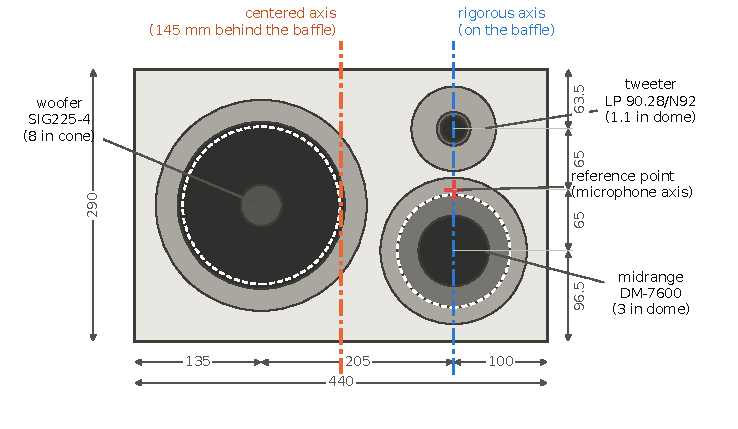
\includegraphics[width=0.86\textwidth]{baffle_front.pdf}
  \caption{Front view of the simulated monitor (dimensions in mm). Dashed white circles: radiators
  used in the model (piston of the woofer's $S_d$, equivalent radiating cap of the midrange).
  Blue: rotation axis of the rigorous setup, on the baffle through midrange and tweeter. Orange:
  rotation axis when the cabinet is centered on the turntable, 145\,mm behind the baffle.}
  \label{fig:front}
\end{figure}

\begin{table}[tbp]
  \centering
  \caption{Driver positions in the speaker frame and radiator models.}
  \label{tab:layout}
  \small
  \begin{tabular}{lccl}
    \toprule
    & $x$ (mm) & $y$ (mm) & radiator \\
    \midrule
    Woofer, Dayton Audio SIG225-4 & $-85$ & $0$ & flat piston, $a=\sqrt{S_d/\pi}=83.8$\,mm \\
    Midrange, HiVi DM-7600 & $120$ & $-48.5$ & equivalent cap, $a=60$\,mm, $h=17.5$\,mm \\
    Tweeter, SICA LP 90.28/N92 & $120$ & $81.5$ & spherical cap, $a=14$\,mm, $h=7.5$\,mm \\
    Reference point $\vect R$ & $120$ & $16.5$ & --- \\
    \bottomrule
  \end{tabular}
\end{table}

\subsection{Driver responses from the datasheets}
\label{sec:datasheets}

Each driver is described by its on-axis half-space response $H_i(f)$: complex pressure at
$r_\text{ref}=1$\,m for 2.83\,V, in an infinite baffle. The SPL curves $L_i(f)$ of the three
datasheets are vector graphics; they were extracted point by point from the PDF files rather than
traced by eye (the CSV files are in the repository). Each curve is taken as the half-space
response, interpolated linearly in $\log f$ and extended outside its published range with fixed
slopes $s_\text{lo}$ and $s_\text{hi}$ (dB per octave):
\begin{equation}
  L(f) = L(f_\text{min}) + s_\text{lo}\log_2\frac{f}{f_\text{min}} \quad (f<f_\text{min}),\qquad
  L(f) = L(f_\text{max}) + s_\text{hi}\log_2\frac{f}{f_\text{max}} \quad (f>f_\text{max}),
\end{equation}
with $s_\text{lo}=+12$ for all three drivers and $s_\text{hi}=-24$ (woofer) or $-12$ (domes). The
magnitude $|H_i|=p_\text{ref}\,10^{L_i/20}$ ($p_\text{ref}=20$\,µPa) is given a minimum phase with
the folded real cepstrum: on an $N$-point DFT grid,
\begin{equation}
  c[n]=\mathrm{IDFT}\{\ln|H[k]|\},\qquad
  \hat c[n]=\begin{cases} c[n] & n=0,\ n=N/2\\ 2c[n] & 0<n<N/2\\ 0 & N/2<n<N\end{cases},\qquad
  H_\text{min}[k]=\exp\big(\mathrm{DFT}\{\hat c\}[k]\big),
  \label{eq:minphase}
\end{equation}
evaluated on a grid eight times finer than the simulation grid to avoid cepstral aliasing.

\paragraph{Woofer in its closed box.} The SIG225-4 datasheet curve is close to an infinite-baffle
response at low frequency (its low end follows $f_s=40$\,Hz, $Q_{ts}=0.43$). It is moved into the
24\,L box with the ratio of the two second-order high-pass functions,
\begin{equation}
  H_\text{woofer}(f)=H_\text{ds}(f)\,\frac{\mathcal H(f;f_c,Q_{tc})}{\mathcal H(f;f_s,Q_{ts})},\qquad
  \mathcal H(f;f_0,Q)=\frac{s^2}{s^2+s/Q+1},\ s=\jj\frac{f}{f_0},
\end{equation}
\begin{equation}
  \alpha=\frac{V_{as}}{V_b}=\frac{29.7}{24},\qquad f_c=f_s\sqrt{1+\alpha}=\fcbox\text{ Hz},\qquad
  Q_{tc}=Q_{ts}\sqrt{1+\alpha}=\qtcbox
\end{equation}
(lossless box). Both high-pass functions are minimum phase, so the product stays minimum phase. As
a check, the Thiele--Small parameters give a mass-controlled sensitivity
\begin{equation}
  p=\frac{\rho_0\,S_d\,Bl\,V}{2\pi r\,R_e\,M_{ms}}=0.75\text{ Pa}\quad(\rho_0=1.204\text{ kg/m}^3),
\end{equation}
that is 91.5\,dB at 1\,m for the datasheet's 91.4\,dB.

\paragraph{Band limit.} All responses are multiplied by a raised-cosine taper from 20.5 to
23.5\,kHz, which keeps the impulse responses band-limited at the 48\,kHz sample rate.

Figure~\ref{fig:models} compares models and datasheets.

\begin{figure}[tbp]
  \centering
  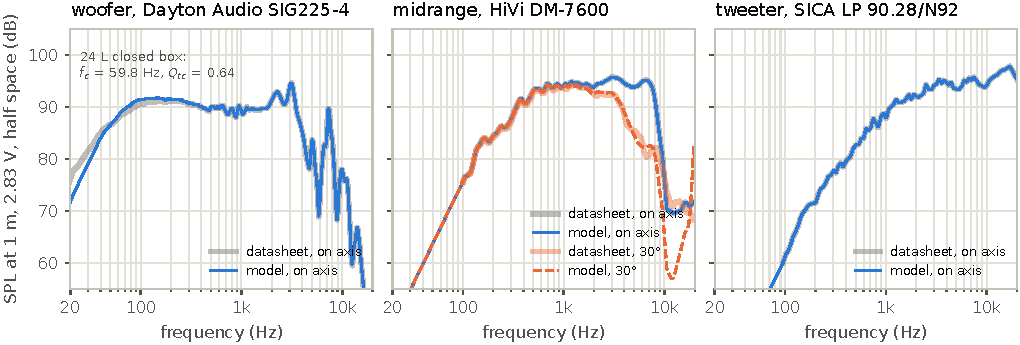
\includegraphics[width=\textwidth]{driver_models.pdf}
  \caption{Driver models against the datasheet curves (half space, 1\,m, 2.83\,V). The woofer is
  shown in its 24\,L closed box. For the midrange, the datasheet also gives the 30$^\circ$ response,
  which the equivalent radiating cap reproduces to within 0.8\,dB RMS between 1.5 and 8\,kHz.}
  \label{fig:models}
\end{figure}

\subsection{Radiators}
\label{sec:radiators}

The directivities are the classical far-field ones \cite{beranek}, normalized to 1 on the driver's
own axis ($\theta$ is the angle from that axis, $k=2\pi f/c$, $c=343$\,m/s).

\paragraph{Cone: rigid flat piston} of radius $a=\sqrt{S_d/\pi}$ in an infinite baffle,
\begin{equation}
  D_\text{p}(\theta,k)=\frac{2J_1(ka\sin\theta)}{ka\sin\theta}.
\end{equation}

\paragraph{Dome: rigid convex spherical cap} of base radius $a$ and height $h$, moving axially. Its
far field is the Rayleigh integral over the projected disc, each ring of radius $r$ being advanced
by the cap height $z(r)$:
\begin{equation}
  A(\theta,k)=\frac{2}{a^2}\int_0^a J_0(kr\sin\theta)\,e^{\jj kz(r)\cos\theta}\,r\dd r,\qquad
  z(r)=\sqrt{R_s^2-r^2}-(R_s-h),\quad R_s=\frac{a^2+h^2}{2h},
  \label{eq:dome}
\end{equation}
\begin{equation}
  D_\text{d}(\theta,k)=\frac{A(\theta,k)}{A(0,k)}.
\end{equation}
$D_\text{d}$ is complex: the protruding center moves the apparent source off axis. With $h=0$ it is
the piston. The integral is evaluated with 96-point Gauss--Legendre quadrature.

\paragraph{The midrange's equivalent cap.} The DM-7600 sits in a horn-shaped aluminum faceplate.
A bare 75\,mm dome is far wider than the datasheet's 30$^\circ$ curve (3\,dB down at 5\,kHz where the
datasheet shows 8\,dB). Fitting $(a,h)$ of Eq.~\eqref{eq:dome} to the datasheet difference
$L_{30^\circ}-L_{0^\circ}$ between 1.5 and 8\,kHz gives $a=60$\,mm, $h=17.5$\,mm (0.83\,dB RMS):
a 120\,mm aperture, the diameter of the faceplate's mouth (the baffle cutout is 120.5\,mm). That
equivalent cap is used for the midrange. The tweeter, with no off-axis data, uses its own
geometry: a 28\,mm silk dome, assumed 7.5\,mm high.

\subsection{Cabinet diffraction: the Distributed Edge Dipole model}

The edges of the front baffle are modelled with the Distributed Edge Dipole (DED) approach of
Urban \emph{et al.}\ \cite{urban2004}, a refinement of the edge-source picture of
Vanderkooy \cite{vanderkooy1991}: a line of dipoles along the edges, driven by the pressure
the driver produces there. In the form used here, extended to a source of finite size, driver $i$
produces at the microphone position $\vect M$
\begin{equation}
  p_i(\vect M,f)=H_i(f)\,\big[P_{\text{dir},i}(\vect M,f)+P_{\text{edge},i}(\vect M,f)\big],
  \label{eq:ded}
\end{equation}
\begin{equation}
  P_{\text{dir},i}=D_i(\theta_i,k)\,\frac{1+\cos\theta_i}{2}\,\frac{r_\text{ref}}{r_i}\,e^{-\jj kr_i},\qquad
  r_i=|\vect M-\vect S_i|,\quad \cos\theta_i=\frac{\vect n\cdot(\vect M-\vect S_i)}{r_i},
\end{equation}
\begin{equation}
  P_{\text{edge},i}=\sum_e Q_{i,e}(f)\,F_e(\vect M)\,\frac{r_\text{ref}}{r_{2,e}}\,e^{-\jj kr_{2,e}},\qquad
  r_{2,e}=|\vect M-\vect E_e|,\quad F_e(\vect M)=-\frac{\vect n\cdot(\vect M-\vect E_e)}{r_{2,e}},
\end{equation}
where $\vect S_i$ is the driver center, $\vect n=\vect e_z$ the baffle normal, $D_i$ the radiator
directivity, and $\vect E_e$, $\Delta l_e$ the midpoints and lengths of the elements along the four
edges of the baffle (2\,mm elements, 730 in all). The factor $(1+\cos\theta)/2$ is the obliquity
of the direct field: 1 on axis, $\tfrac12$ in the baffle plane, 0 behind; $F_e$ is the edge dipole,
zero in the baffle plane and changing sign behind it. The strength of edge element $e$ is
\begin{equation}
  Q_{i,e}(f)=C_i\,\Delta l_e\,\frac{G_i(\rho_{i,e},f)}{A_i(0,k)},\qquad
  G_i(\rho,f)=\frac{1}{S_i}\iint_{S_i}\frac{1+\cos\theta_s}{2}\,\frac{e^{-\jj kr_1}}{r_1}\dd S,
  \label{eq:edge}
\end{equation}
where the integral runs over the radiating surface (the projected disc, each point raised by the
cap height $z(r)$ for a dome), $r_1$ is the distance from the surface point to the edge point,
$\cos\theta_s=-z(r)/r_1$ the obliquity toward it, $\rho_{i,e}=|\vect E_e-\vect S_i|$, and $A_i(0,k)$
(Eq.~\ref{eq:dome}; 1 for a piston) refers the edge drive to the on-axis level that $H_i$
describes. The constant
\begin{equation}
  C_i=\frac{1}{2\sum_e\Delta l_e\,G_i(\rho_{i,e},0)}
\end{equation}
makes $P_\text{dir}+P_\text{edge}=\tfrac12$ on axis in the far field at low frequency: the cabinet
radiates 6\,dB below the half-space response at low frequency (full-space radiation) and reaches it
at high frequency --- the baffle step.

All paths keep their true length: the edge waves arrive $(r_1+r_2-r)/c$ after the direct sound,
\emph{at the actual microphone position}. That finite-distance geometry is exactly what a
point-source correction cannot reproduce, and the reason for using the DED model here. As in the
DED formulation, only the edges of the face that carries the drivers are modelled; behind the
baffle the field is the sum of the edge dipoles plus the vanishing direct term.

\paragraph{Numerics.} $G_i(\rho,f)\,e^{\jj k\rho}$ varies slowly with $\rho$ and $f$ once the
common delay $\rho/c$ is removed. It is tabulated on a 1\,mm grid of $\rho$ and a 50\,Hz grid of
$f$, with a Gauss--Legendre rule in $r$ and a midpoint rule in azimuth over half a turn (the
integrand is even), sized for the phase spread $2k_\text{max}a$ across the surface ($n_r=\lceil
0.7\cdot2k_\text{max}a+16\rceil$, $n_\varphi=\lceil 0.5\cdot2k_\text{max}a+16\rceil$); it is then
interpolated linearly in $\rho$ and with cubic splines in $f$. On each driver's axis at 30\,m,
$P_\text{dir}+P_\text{edge}$ is at $-5.97$\,dB at 20\,Hz for all three drivers, and within 0.3\,dB of
0\,dB at 10\,kHz.

\begin{figure}[tbp]
  \centering
  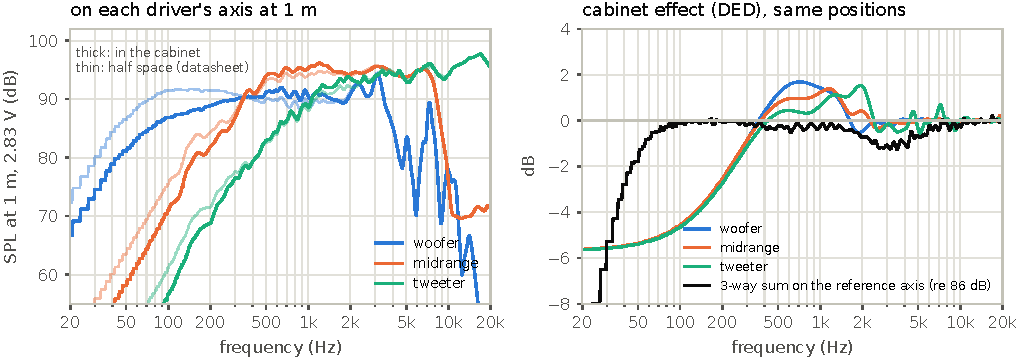
\includegraphics[width=\textwidth]{inbox_onaxis.pdf}
  \caption{Left: each driver on its own axis at 1\,m, in the cabinet (thick) and in half space
  (thin). Right: their ratio, the cabinet effect according to the DED model (baffle step and
  edge ripple), and the illustrative three-way sum on the reference axis.}
  \label{fig:inbox}
\end{figure}

\subsection{An illustrative three-way crossover}
\label{sec:crossover}

To look at the summed loudspeaker, each driver is equalized to an acoustic target on the reference
axis at 1\,m (rigorous setup):
\begin{equation}
  T_\text{woofer}=\mathrm{LR}_4^\text{LP}(450)\,\mathrm{B}_2^\text{HP}(40),\quad
  T_\text{mid}=\mathrm{LR}_4^\text{HP}(450)\,\mathrm{LR}_4^\text{LP}(3000),\quad
  T_\text{tweeter}=\mathrm{LR}_4^\text{HP}(3000),
\end{equation}
with $\mathrm{B}_2^\text{LP}(f_0)=1/(s^2+\sqrt2 s+1)$, $\mathrm{B}_2^\text{HP}=s^2/(s^2+\sqrt2s+1)$,
$s=\jj f/f_0$, and $\mathrm{LR}_4=\mathrm{B}_2^2$. The filter of driver $i$ is the minimum-phase filter
(Eq.~\ref{eq:minphase}) with magnitude $L\,|T_i|/S_i$, where $S_i$ is the 1/6-octave smoothed on-axis
magnitude of the driver and $L$ corresponds to 86\,dB SPL. The summed response is
$p_\text{sys}=\sum_i X_i\,p_i$. The same filters are used in every case: only the measurements change.
The design is not optimized (Figure~\ref{fig:inbox}, right) and does not need to be.

% =============================================================================================
\section{Measurement geometry}

\subsection{Turntable kinematics}

The turntable axis is vertical, at $\vect A=(a_x,\cdot,a_z)$ in the speaker frame. The microphone is
fixed in the room; at $0^\circ$ it is on the reference axis, at distance $d$ from the baffle:
$\vect M_0=(x_R,\,y_R,\,d)$. Turning the loudspeaker by $\theta$ moves the microphone, seen from the
loudspeaker, by $-\theta$ about the axis. With positive angles bringing the microphone toward $+x$
(the midrange/tweeter side):
\begin{equation}
  \begin{aligned}
    x(\theta)&=a_x+(x_R-a_x)\cos\theta+(d-a_z)\sin\theta,\\
    z(\theta)&=a_z-(x_R-a_x)\sin\theta+(d-a_z)\cos\theta,
  \end{aligned}\qquad y(\theta)=y_R.
  \label{eq:kinematics}
\end{equation}
\begin{itemize}
  \item \textbf{Rigorous setup}: $\vect A$ on the reference point, $(a_x,a_z)=(x_R,0)$. The microphone
  stays on the circle of radius $d$ around $\vect R$: $(x,z)=(x_R+d\sin\theta,\ d\cos\theta)$.
  \item \textbf{Centered setup}: the cabinet is centered on the turntable, $(a_x,a_z)=(0,-D/2)$, i.e.
  145\,mm behind the baffle and 120\,mm to the left of the reference axis. The microphone has been
  moved 120\,mm sideways so that it faces the reference point at $0^\circ$
  (Figures~\ref{fig:3d} and~\ref{fig:top}).
\end{itemize}

\begin{figure}[tbp]
  \centering
  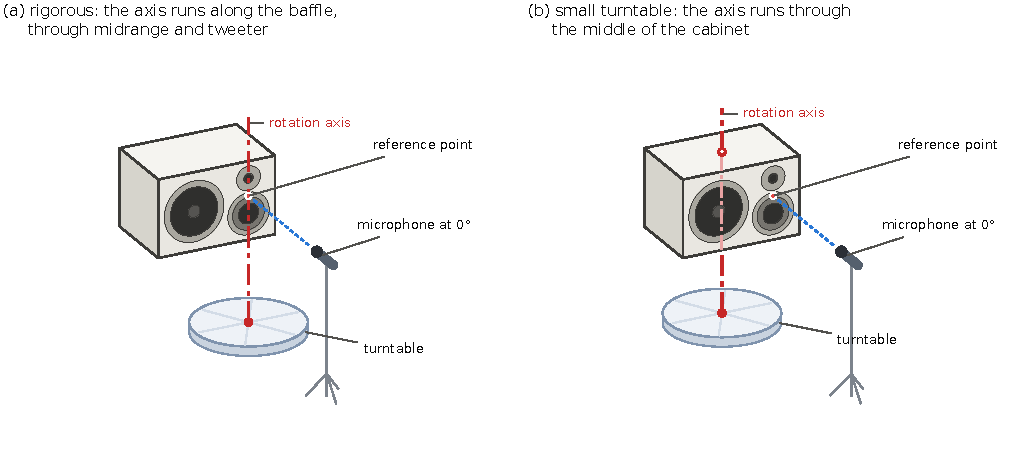
\includegraphics[width=\textwidth]{setups_3d.pdf}
  \caption{The two setups, with the loudspeaker raised above the disc that stands for the
  turntable. Dash-dotted red: the rotation axis --- (a) along the baffle, through the midrange and
  the tweeter; (b) through the middle of the cabinet (lighter where it is hidden inside the box).
  The microphone faces the reference point (red dot) at $0^\circ$ in both cases.}
  \label{fig:3d}
\end{figure}

\begin{figure}[tbp]
  \centering
  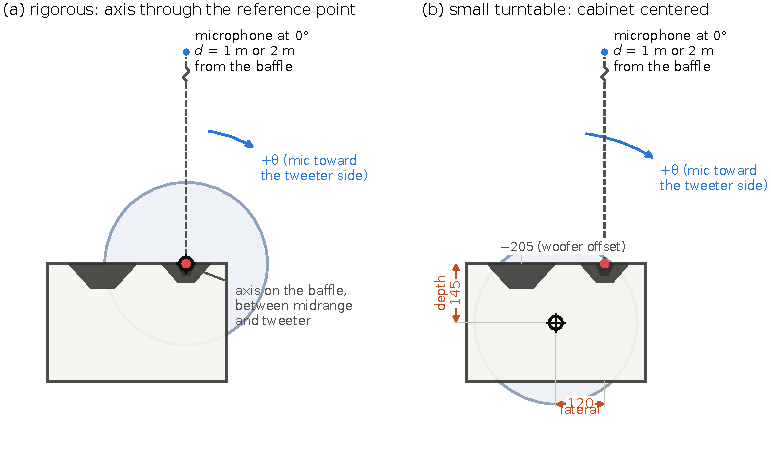
\includegraphics[width=\textwidth]{setups_top.pdf}
  \caption{Top views to scale (turntable 400\,mm across; microphone distance not to scale). In (b)
  the correction needs the depth (rotation axis to baffle, 145\,mm), the lateral offset (rotation axis
  to reference axis, $+120$\,mm, positive toward the side the microphone faces at $+90^\circ$), each
  driver's offset from the reference axis ($-205$\,mm for the woofer, 0 for midrange and tweeter)
  and the microphone distance.}
  \label{fig:top}
\end{figure}

\subsection{What the raw measurement gets wrong}

Seen from a driver at $\vect S$, the microphone of the centered setup is at a distance
$\rho_k=|\vect M(\theta_k)-\vect S|$ and in a direction $\varphi_k$ that differ from the intended ones
(Figure~\ref{fig:positions}). Figure~\ref{fig:kinematics} and Table~\ref{tab:kinematics} give the
consequences in the horizontal plane: the raw off-axis responses are up to 2.5--2.8\,dB too low and
almost 1\,ms late behind the cabinet at 1\,m, and the direction is wrong by up to 15$^\circ$. At 2\,m the
level and direction errors halve; the delay does not (it is set by the axis offset, not by the
distance).

\begin{figure}[tbp]
  \centering
  \begin{minipage}{0.42\textwidth}
    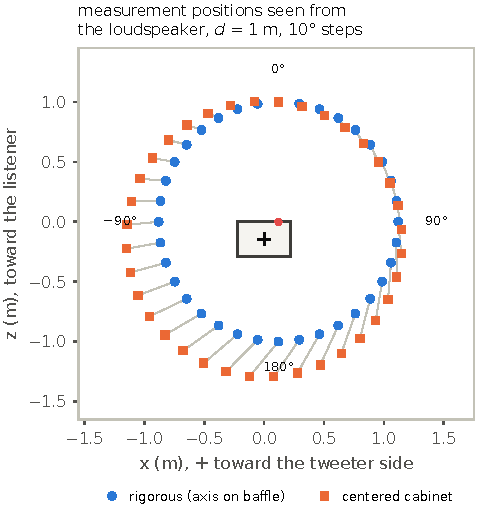
\includegraphics[width=\textwidth]{positions_to_scale.pdf}
  \end{minipage}\hfill
  \begin{minipage}{0.55\textwidth}
    \caption{Microphone positions relative to the loudspeaker, to scale, at 1\,m. Blue: rigorous
    setup, a circle of 1\,m around the reference point. Orange: centered setup, a circle of 1.15\,m
    around the middle of the cabinet. Gray segments join the positions with the same nominal angle.}
    \label{fig:positions}
  \end{minipage}
\end{figure}

\begin{figure}[tbp]
  \centering
  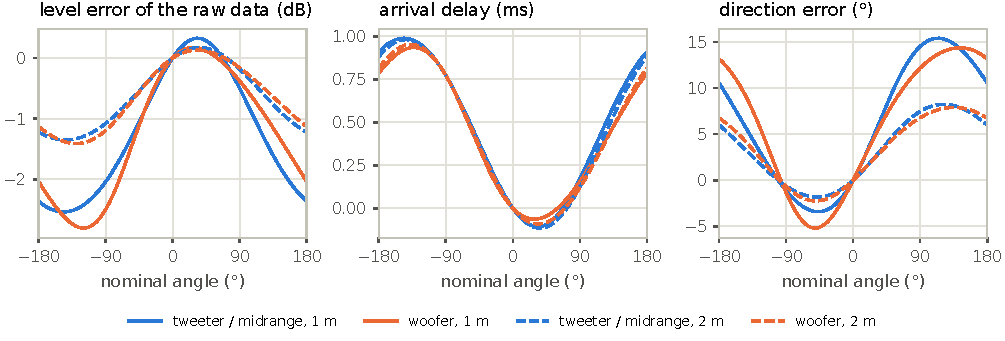
\includegraphics[width=\textwidth]{kinematics.pdf}
  \caption{Errors of the raw measurement in the centered setup, seen from the drivers: level
  ($20\log_{10}$ of the distance ratio), extra arrival delay and direction error, against the nominal
  angle.}
  \label{fig:kinematics}
\end{figure}

\begin{table}[tbp]
  \centering
  \caption{Range of the geometric errors of the raw measurement (centered setup).}
  \label{tab:kinematics}
  \begin{tabular}{llccc}
    \toprule
    driver & $d$ & level (dB) & delay (ms) & direction ($^\circ$) \\
    \midrule
    \rows{kinematics}
    \bottomrule
  \end{tabular}
\end{table}

% =============================================================================================
\section{The correction method}

The correction rebuilds, for each nominal angle, the response that would have been measured at
the ideal position. It works plane by plane and driver by driver.

\subsection{Inputs and geometry}

In the plane of rotation, take a frame with the rotation axis at the origin, $y$ toward the front
and $x$ toward the \emph{+ side} (the side the microphone faces at $+90^\circ$). The user provides
\begin{itemize}
  \item the depth $\delta$: from the rotation axis to the baffle (positive when the axis is behind it);
  \item the lateral offset $\ell$: from the rotation axis to the reference axis, positive toward the
  + side;
  \item the driver offset $o$: from the reference axis to the driver, positive toward the + side;
  \item the microphone distance $r_0$ from the baffle at $0^\circ$.
\end{itemize}
Then the reference point is $\vect R=(\ell,\delta)$, the driver $\vect S=\vect R+(o,0)$, and
\begin{align}
  \text{measured position:}\quad &\vect M_k=\mathcal R(\theta_k)\,(\ell,\ \delta+r_0),\\
  \text{ideal position:}\quad &\vect M^*(\theta)=\vect R+r_0(\sin\theta,\ \cos\theta),
\end{align}
with the rotation $\mathcal R(\theta)(x,y)=(x\cos\theta+y\sin\theta,\ -x\sin\theta+y\cos\theta)$
(positive angles toward the + side).
The 0$^\circ$ measurement is on the reference axis, $\ell$ away from the rotation axis: the lateral
shift of the microphone is part of the model. Seen from the driver, every position has a direction
and a distance,
\begin{equation}
  \varphi=\operatorname{atan2}(M_x-S_x,\ M_y-S_y)\ \ (\text{unwrapped to within }\pi\text{ of }\theta),\qquad
  \rho=|\vect M-\vect S|.
\end{equation}
For the setup of Figure~\ref{fig:top}(b): $\delta=145$\,mm, $\ell=+120$\,mm, $o=-205$\,mm for the
woofer and 0 for the midrange and tweeter, $r_0=1000$ or 2000\,mm.

\subsection{Point-source re-propagation}

Around each driver the response is assumed to be that of a point source with a directivity,
\begin{equation}
  h(\varphi,\rho,t)=\frac{g(\varphi,\,t-\rho/c)}{\rho},
\end{equation}
so a measurement taken at $(\varphi_k,\rho_k)$ is moved to the target distance $\rho^*$ by a delay
and a gain:
\begin{equation}
  h_{k\to*}(t)=\frac{\rho_k}{\rho^*}\;h_k\!\left(t-\frac{\rho^*-\rho_k}{c}\right).
\end{equation}

\subsection{Angular interpolation}

The measurements, sorted by $\varphi_k$, serve as supports (for a full circle, copies at
$\varphi_k\pm2\pi$ close the loop). For the target direction $\varphi^*$ the two bracketing supports
$a$, $b$ are interpolated linearly \emph{after} both have been moved to $\rho^*$, so that they are in
time and do not comb-filter:
\begin{equation}
  h^*(t)=(1-u)\,h_{a\to*}(t)+u\,h_{b\to*}(t),\qquad u=\frac{\varphi^*-\varphi_a}{\varphi_b-\varphi_a}.
\end{equation}
Outside the measured range the nearest support is used. The $0^\circ$ measurement is the reference and
is never changed. A measurement copied by symmetry at $-\theta$ stands for the mirror image of the one
at $\theta$ and is placed at $(-\varphi_k,\rho_k)$ of that one.

\subsection{Implementation}

The fractional delays are applied as linear phases. With $\tau_k=(\rho^*-\rho_k)f_s/c$ samples,
$p=\lceil\max|\tau_k|\rceil+1$ samples of margin and an FFT length $N_c=2^{\lceil\log_2(L+2p+64)\rceil}$
($L$ the longest impulse response),
\begin{equation}
  H^*[m]=\sum_{\text{supports}} g_k\,X_k[m]\,e^{-\jj2\pi\tilde m(\tau_k+p)/N_c},\qquad
  \tilde m=\begin{cases}m & m\le N_c/2\\ m-N_c & m>N_c/2\end{cases},
\end{equation}
with $g_k$ the interpolation weight times $\rho_k/\rho^*$ and $X_k$ the DFT of the zero-padded
measurement; the corrected impulse response is $\mathrm{Re}\,\mathrm{IDFT}\{H^*\}$ from sample $p$ on.

\subsection{Assumptions}

The method assumes a point source on the baffle plane whose far-field directivity does not depend on
distance, and ignores what is outside the plane of rotation. The cabinet edges violate the first
assumption; the vertical offsets between drivers and microphone (here $\pm65$\,mm for the domes),
the third.

% =============================================================================================
\section{Simulation protocol}

\paragraph{Measurements.} Horizontal orbit from $-180^\circ$ to $180^\circ$ in $10^\circ$ steps
(36 positions; $\pm180^\circ$ is one position), microphone at $d=1$\,m and $d=2$\,m from the baffle, at
the reference height. For every position, Eq.~\eqref{eq:ded} gives the complex spectrum of each driver
on a 16\,384-point grid at 48\,kHz (2.93\,Hz resolution); the impulse responses are its inverse
real FFT (341\,ms, far longer than any delay or decay).

\paragraph{Cases.}
\begin{itemize}
  \item \textbf{rigorous}: axis on the reference point --- the reference;
  \item \textbf{uncorrected}: cabinet centered, microphone moved onto the reference axis;
  \item \textbf{corrected}: the same data after the correction with the true parameters;
  \item \textbf{direct sound only}: the three cases again with $P_\text{edge}=0$, to separate the
  correction's own errors from those due to diffraction;
  \item \textbf{variants}: corrected with wrong parameters (lateral offset omitted or with the wrong
  sign, woofer offset omitted, depth or lateral offset off by $\pm10$\,mm, microphone distance off by
  $+20$\,mm), and with a $5^\circ$ orbit.
\end{itemize}

\paragraph{Metrics.} Power spectra are smoothed to 1/24 octave,
\begin{equation}
  P_X(\theta,f)=\big\langle|p_X(\theta,f')|^2\big\rangle_{f'\in[f\,2^{-1/48},\,f\,2^{1/48}]},
\end{equation}
and compared with the rigorous case through the level error
\begin{equation}
  \Delta L_X(\theta,f)=10\log_{10}\frac{P_X(\theta,f)}{P_\text{rigorous}(\theta,f)}\ \text{dB}.
\end{equation}
Statistics (RMS, 95th percentile, maximum of $|\Delta L|$) are taken over the points that matter: in
the driver's band (woofer 50\,Hz--1\,kHz, midrange 300\,Hz--6\,kHz, tweeter 2--20\,kHz, summed
loudspeaker 50\,Hz--20\,kHz), and no more than 20\,dB below the rigorous on-axis response at the same
frequency (this leaves out the deep nulls of a beaming cone, where a fraction of a degree changes the
level by tens of dB).

\paragraph{CTA-2034-A curves from the horizontal orbit.} Only the horizontal orbit is measured, so the
standard's curves \cite{cta2034} are estimated from it (all averages on squared pressures):
\begin{align}
  \mathrm{LW}^2&=\tfrac17\textstyle\sum_{\theta\in\{0,\pm10,\pm20,\pm30\}}|p(\theta)|^2,\\
  \mathrm{ER}^2&=\tfrac13\big(\mathrm{FW}^2+\mathrm{SW}^2+\mathrm{RW}^2\big),\\
  \mathrm{SP}^2&=\frac{\sum_\theta w(\theta)\,|p(\theta)|^2}{\sum_\theta w(\theta)},\\
  \mathrm{PIR}^2&=0.12\,\mathrm{LW}^2+0.44\,\mathrm{ER}^2+0.44\,\mathrm{SP}^2,\qquad
  \mathrm{DI}=10\log_{10}\frac{\mathrm{LW}^2}{\mathrm{SP}^2},
\end{align}
where the front-wall (FW), side-wall (SW) and rear-wall (RW) groups are themselves RMS averages
over the angles $0$, $\pm10$, $\pm20$, $\pm30^\circ$ (FW), $\pm40$ to $\pm80^\circ$ (SW) and $\pm90$,
$180^\circ$ (RW). The standard adds the
$\pm10^\circ$ vertical directions to the listening window and the floor and ceiling bounces (vertical
orbit) to the early reflections; using the horizontal weights alone for the sound power amounts to
assuming the vertical orbit equal to the horizontal one. The sound-power weights are those of the
standard's Appendix C,
\begin{equation}
  w(\theta)=\Omega(\theta+5^\circ)-\Omega(\theta-5^\circ),\qquad \Omega(\alpha)=4C-2\pi,
\end{equation}
with $\Omega(\alpha)$ the solid angle of the spherical square bounded by the great circles at $\pm\alpha$ horizontally and
vertically ($C$ its corner angle), symmetric about $90^\circ$ and doubled at $90^\circ$
(Table~\ref{tab:weights}). These estimates are the same for every case, so their differences measure
the measurement geometry only.

\begin{table}[tbp]
  \centering
  \caption{Sound-power weights of the horizontal orbit (CTA-2034-A Appendix C), normalized over the
  36 directions; $w(180^\circ-\theta)=w(\theta)$.}
  \label{tab:weights}
  \begin{tabular}{cccccccccc}
    \toprule
    \rows{weights}
    \bottomrule
  \end{tabular}
\end{table}

% =============================================================================================
\section{Results}

\subsection{Uncorrected: what the centered setup does to the data}

Figure~\ref{fig:maps} (center column) and Figure~\ref{fig:selected1} show the uncorrected data
against the rigorous ones. Off axis the responses are too low --- by the distance ratio, up to
2.5\,dB behind the cabinet at 1\,m --- and, where the response changes quickly with angle (beaming
of the woofer and of the midrange's horn-loaded dome, diffraction ripple behind the cabinet), they
show features of the wrong direction. Within the relevant points the summed loudspeaker is off by
\sysRawOne\,dB RMS at 1\,m and \sysRawTwo\,dB at 2\,m (Table~\ref{tab:errors}).

\begin{figure}[tbp]
  \centering
  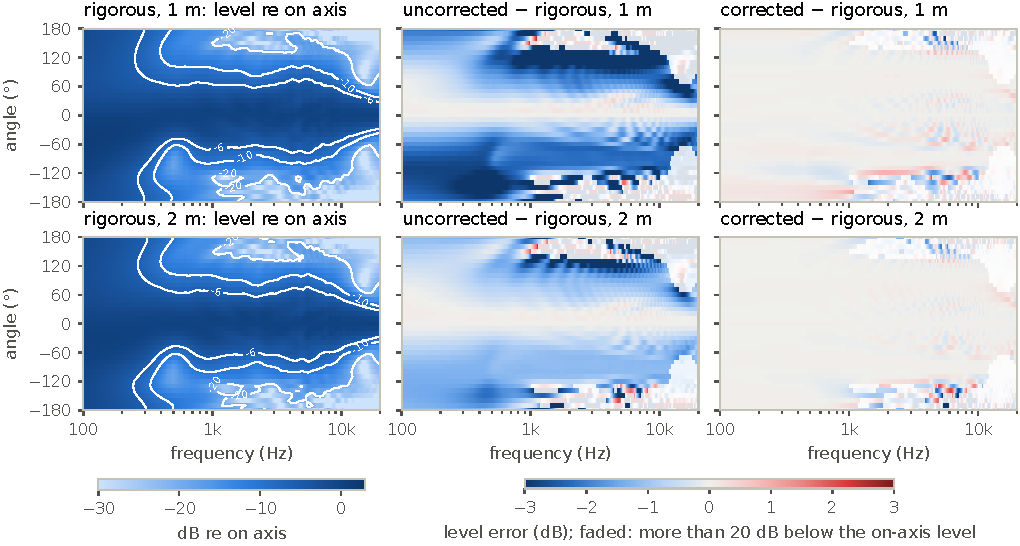
\includegraphics[width=\textwidth]{system_maps.pdf}
  \caption{Summed loudspeaker. Left: rigorous horizontal polar map, normalized to the on-axis
  response (contours at $-6$, $-10$, $-20$\,dB). Center and right: level error of the uncorrected and
  corrected data; points more than 20\,dB below the on-axis level are faded.}
  \label{fig:maps}
\end{figure}

\begin{figure}[tbp]
  \centering
  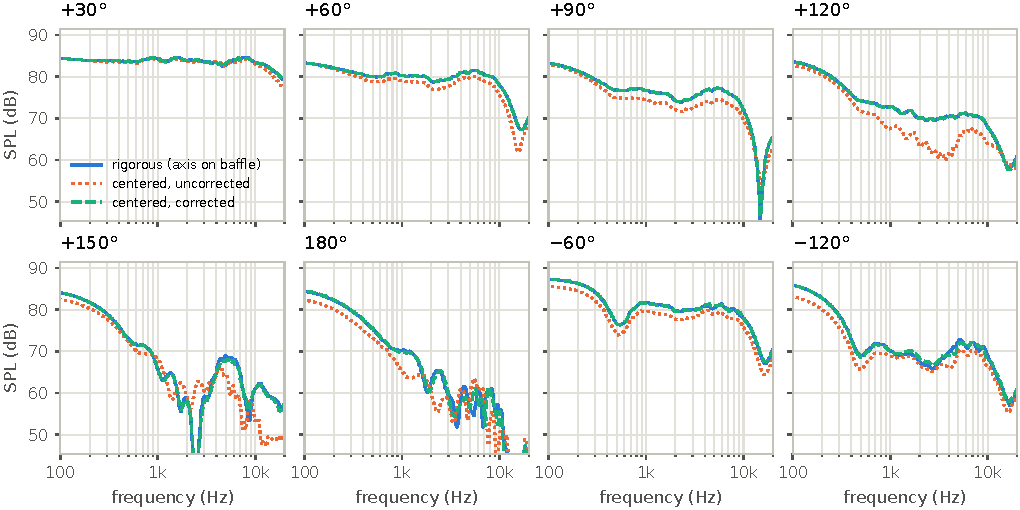
\includegraphics[width=\textwidth]{selected_system_1m.pdf}
  \caption{Summed loudspeaker at selected angles, 1\,m, 1/12-octave smoothing.}
  \label{fig:selected1}
\end{figure}

\subsection{Corrected, direct sound only: the method itself}

Without edge diffraction every driver is exactly a point source with a directivity, as the
correction assumes. What remains is the interpolation between measured directions and the vertical
offsets that the planar model ignores: 0.02--0.08\,dB RMS and 0.6\,dB at worst
(Table~\ref{tab:errors}, ``direct only''). Moving every driver to the microphone height changes the RMS
figures by less than 0.01\,dB: the out-of-plane offsets are negligible at 1\,m and beyond. In this
idealized world the correction is, for practical purposes, exact.

\begin{table}[tbp]
  \centering
  \caption{Level error $|\Delta L|$ against the rigorous measurement over the relevant points (dB): RMS,
  95th percentile and maximum.}
  \label{tab:errors}
  \small
  \begin{tabular}{lllcccccc}
    \toprule
    & & & \multicolumn{3}{c}{uncorrected} & \multicolumn{3}{c}{corrected}\\
    \cmidrule(lr){4-6}\cmidrule(lr){7-9}
    $d$ & model & driver & RMS & p95 & max & RMS & p95 & max\\
    \midrule
    \rows{errors}
    \bottomrule
  \end{tabular}
\end{table}

\subsection{Corrected, with diffraction: the open question}

With the cabinet edges, the residual grows: \twCorOne\,dB RMS for the tweeter and \sysCorOne\,dB for
the summed loudspeaker at 1\,m, with local deviations up to \twmaxCorOne\,dB (Table~\ref{tab:errors},
Figures~\ref{fig:errmaps1} and~\ref{fig:errmaps2}). Figure~\ref{fig:residuals} shows where: in the
front half ($|\theta|\le90^\circ$) no angle exceeds 0.3\,dB RMS (0.2\,dB for the summed loudspeaker);
the residual is behind the cabinet ($|\theta|\ge120^\circ$), at mid and high frequencies, where the edge
waves dominate the response --- up to 1.3\,dB RMS at one angle for the tweeter at 1\,m, 3\,dB at
2\,m. The
woofer, whose band is low, is hardly affected.

Two mechanisms are at work. First, the edges are not at the driver: the correction moves the edge
waves by the driver's change of distance, not by their own, so their timing relative to the direct
sound keeps the error of the measured position --- visible in the late part of the impulse responses
(Figure~\ref{fig:impulses}). This error shrinks with distance. Second, behind the cabinet the response
is an interference pattern of many edge waves, with lobes about $10^\circ$ wide at 5\,kHz
($\lambda/W$) and narrower above; the correction interpolates between measured directions $10^\circ$
apart, which cannot follow it. This one
does not shrink with distance: at 2\,m the summed loudspeaker keeps \sysCorTwo\,dB RMS and its worst
local deviation even grows to \sysmaxCorTwo\,dB, in a narrow region near $-170^\circ$ around 5--6\,kHz.

\begin{figure}[tbp]
  \centering
  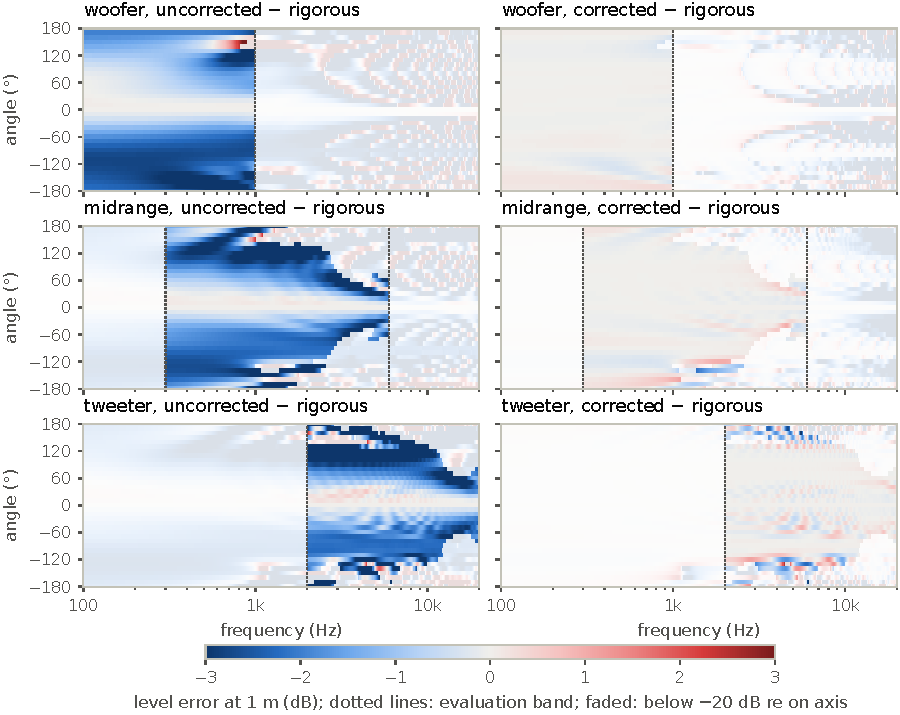
\includegraphics[width=0.92\textwidth]{driver_error_maps_1m.pdf}
  \caption{Level error of each driver at 1\,m, uncorrected (left) and corrected (right). Dotted lines:
  evaluation band. Faded: more than 20\,dB below the on-axis response.}
  \label{fig:errmaps1}
\end{figure}

\begin{figure}[tbp]
  \centering
  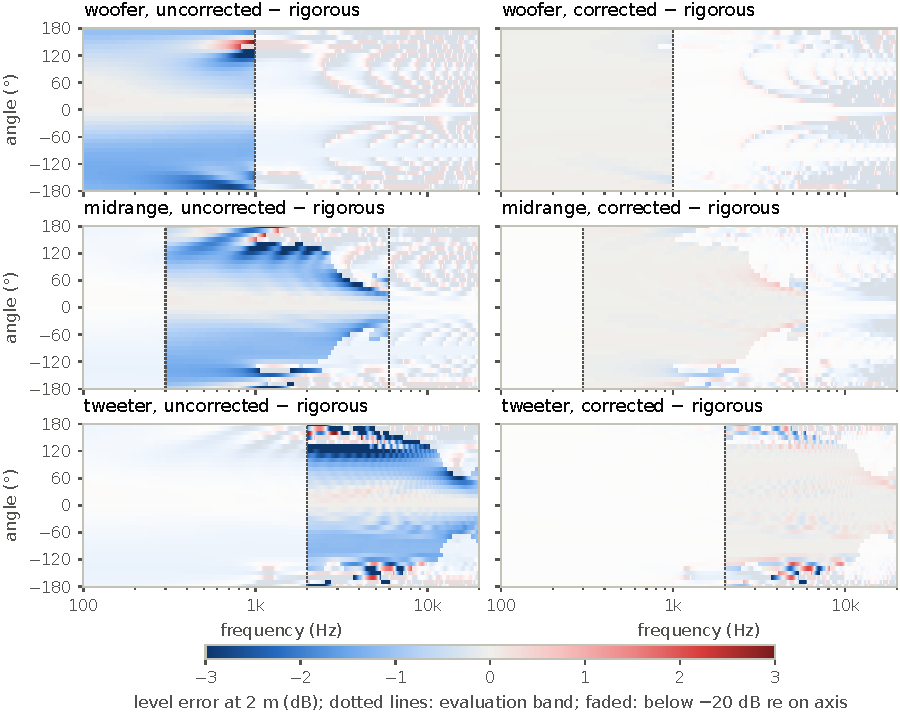
\includegraphics[width=0.92\textwidth]{driver_error_maps_2m.pdf}
  \caption{Same as Figure~\ref{fig:errmaps1} at 2\,m.}
  \label{fig:errmaps2}
\end{figure}

\begin{figure}[tbp]
  \centering
  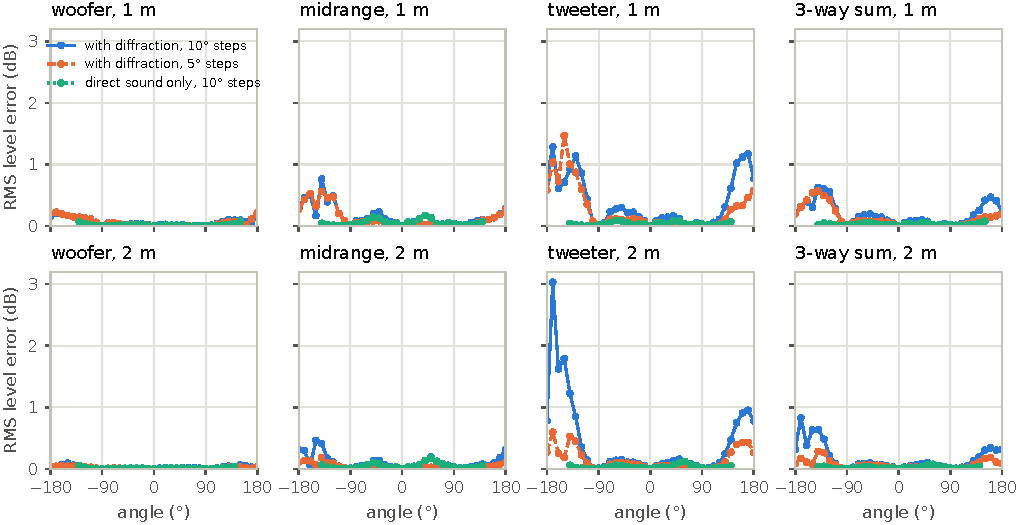
\includegraphics[width=\textwidth]{residuals.pdf}
  \caption{RMS level error of the corrected data at each angle (over the relevant frequencies), with
  the DED diffraction and $10^\circ$ or $5^\circ$ steps, and for the direct sound alone.}
  \label{fig:residuals}
\end{figure}

\begin{figure}[tbp]
  \centering
  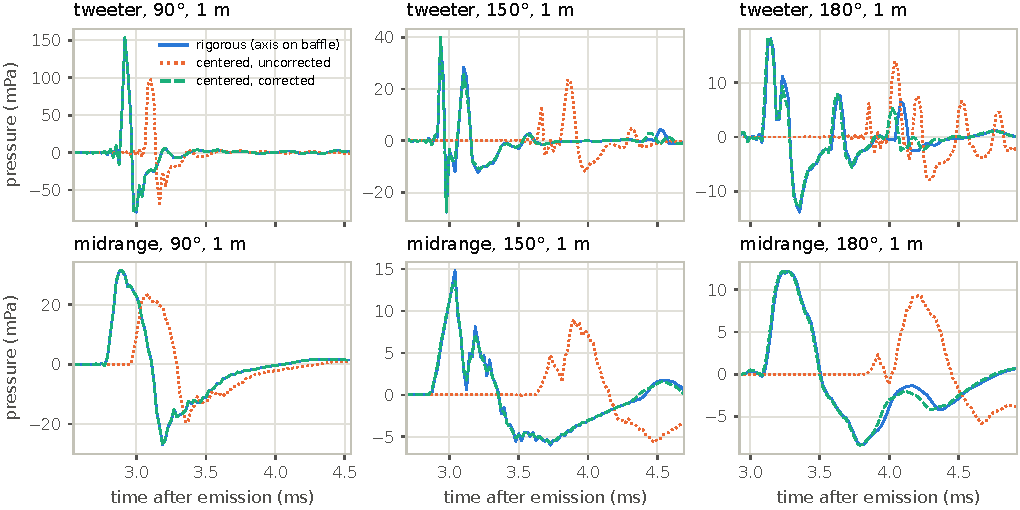
\includegraphics[width=\textwidth]{impulses.pdf}
  \caption{Impulse responses at 1\,m (time from emission). The uncorrected responses arrive late and
  low; the corrected ones line up with the rigorous ones, except for the later edge-wave arrivals
  behind the cabinet.}
  \label{fig:impulses}
\end{figure}

\subsection{Angular resolution}

Halving the step to $5^\circ$ addresses the second mechanism. At 2\,m it brings the summed loudspeaker
from \sysCorTwo\ to \sysFiveTwo\,dB RMS and its worst deviation from \sysmaxCorTwo\ to
\sysmaxFiveTwo\,dB; the tweeter goes from \twCorTwo\ to \twFiveTwo\,dB RMS. At 1\,m the gain is smaller
(\sysCorOne\ to \sysFiveOne\,dB RMS), because there the first mechanism, which no angular step can
fix, takes a larger share.

\subsection{Spatial averages and Predicted In-Room Response}

The CTA-2034-A curves average many directions and the residual errors, concentrated behind the
cabinet and changing sign from one frequency to the next, largely cancel (Figure~\ref{fig:pir},
Table~\ref{tab:cta}). Uncorrected, the centered setup lowers the sound power by up to 1.4\,dB at 1\,m
(every off-axis microphone position is farther away), the PIR by up to \pirRawOne\,dB and shifts the
directivity index by 1.2\,dB; at 2\,m these errors halve. Corrected, the PIR stays within
\pirCorOne\,dB (1\,m) and \pirCorTwo\,dB (2\,m) of the rigorous one, the sound power within 0.13\,dB and
the directivity index within 0.11\,dB.

\begin{figure}[tbp]
  \centering
  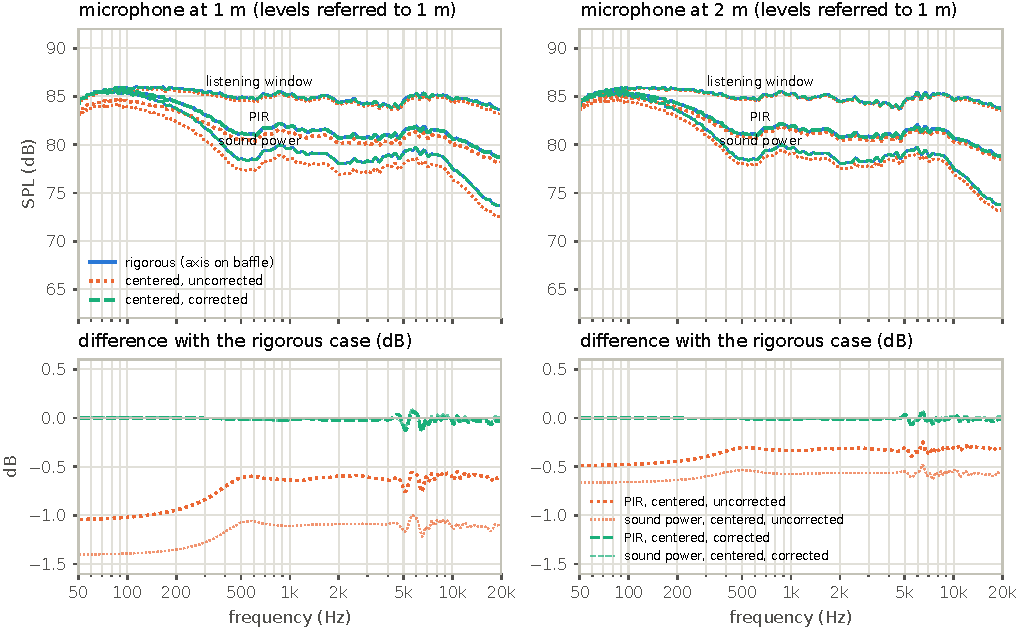
\includegraphics[width=\textwidth]{pir.pdf}
  \caption{Top: listening window, PIR and sound power of the summed loudspeaker from the horizontal
  orbit (levels referred to 1\,m). The corrected curves lie on the rigorous ones. Bottom: differences
  with the rigorous case.}
  \label{fig:pir}
\end{figure}

\begin{table}[tbp]
  \centering
  \caption{Largest deviation from the rigorous case, 100\,Hz--20\,kHz, of the horizontal-orbit
  CTA-2034-A curves of the summed loudspeaker (dB).}
  \label{tab:cta}
  \begin{tabular}{lllccccc}
    \toprule
    $d$ & model & data & LW & ER & SP & PIR & DI\\
    \midrule
    \rows{cta}
    \bottomrule
  \end{tabular}
\end{table}

\subsection{Wrong parameters and the laterally shifted microphone}
\label{sec:variants}

The correction needs the geometry it is given (Figure~\ref{fig:sensitivity}, Table~\ref{tab:variants}).
Errors of $\pm10$\,mm on the depth or the lateral offset, or of 20\,mm on the microphone distance,
change the RMS errors by a few hundredths of a dB and the PIR by less than 0.1\,dB: measuring with a
tape is good enough.

The lateral offset itself is another matter. Because the microphone has been moved sideways to face
the reference point, the model must know that the reference axis is $\ell=120$\,mm from the rotation
axis, on the + side. Omitting it ($\ell=0$, i.e.\ correcting only for the depth, as for a symmetric
loudspeaker) leaves the summed loudspeaker \sysLatZeroOne\,dB RMS off at 1\,m and the PIR up to
\pirLatZeroOne\,dB off; entering it with the wrong sign is as bad (\pirLatSignOne\,dB). For the PIR,
and for the tweeter (\twLatZeroOne\ and \twLatSignOne\,dB RMS against \twRawOne\,dB), both are worse
than no correction at all (\pirRawOne\,dB). The sign convention matters: $\ell$ is positive when the
reference axis lies on the side the microphone faces at $+90^\circ$. With the convention of this study
(positive angles toward the tweeter side) the reference axis is on the + side; a turntable that
counts angles the other way needs $\ell=-120$\,mm and a woofer offset of $+205$\,mm.

The woofer's own offset ($-205$\,mm) matters less: omitting it raises the woofer's error from
\wfCorOne\ to 0.27\,dB RMS (1.7\,dB at worst) at 1\,m, and the summed loudspeaker hardly notices, the
woofer being crossed over at 450\,Hz where its directivity varies slowly.

\begin{figure}[tbp]
  \centering
  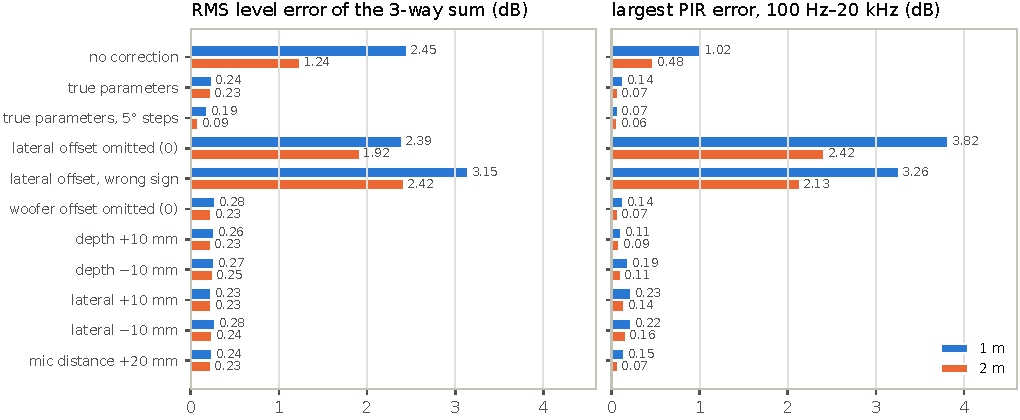
\includegraphics[width=\textwidth]{sensitivity.pdf}
  \caption{Effect of the correction parameters: RMS level error of the summed loudspeaker (left) and
  largest PIR deviation (right), at 1\,m and 2\,m.}
  \label{fig:sensitivity}
\end{figure}

\begin{table}[tbp]
  \centering
  \caption{RMS level error per driver and for the summed loudspeaker, and largest PIR deviation, for
  the correction variants (dB).}
  \label{tab:variants}
  \small
  \setlength{\tabcolsep}{4.5pt}
  \begin{tabular}{lccccc@{\hspace{12pt}}ccccc}
    \toprule
    & \multicolumn{5}{c}{1\,m} & \multicolumn{5}{c}{2\,m}\\
    \cmidrule(lr){2-6}\cmidrule(lr){7-11}
    & woofer & mid & tweeter & sum & PIR & woofer & mid & tweeter & sum & PIR\\
    \midrule
    \rows{variants}
    \bottomrule
  \end{tabular}
\end{table}

% =============================================================================================
\section{A boundary-element check}
\label{sec:bem}

Two parts of the model are approximations, and both matter most where the residual of the correction
lives: the drivers radiate as points with a far-field directivity, and the DED model represents the
cabinet by dipoles along the front edges only, which describes the field behind the cabinet least
well. This section repeats the study on a variant of the loudspeaker computed with the
boundary-element method (BEM), which solves the radiation of the whole cabinet --- every face and
edge, the drivers as extended rigid surfaces --- with neither approximation, from 20\,Hz to 16\,kHz.

\subsection{A two-way variant}

The BEM model is a two-way in the same cabinet (Figure~\ref{fig:bemmodel}): the SIG225-4 woofer at
$x=-85$\,mm and the SICA tweeter at $x=+120$\,mm, both at mid-height ($y=0$). Dropping the midrange
removes a source and, with both drivers on the cabinet's horizontal middle plane, makes the problem
symmetric about the plane of the horizontal orbit, which halves it. The reference point is the
tweeter center and the microphone is at its height: both drivers lie in the plane of rotation. The
correction's parameters are those of the three-way: depth 145\,mm, lateral offset $+120$\,mm, woofer
offset $-205$\,mm, tweeter offset 0.

The radiators are rigid and move along their axis: the woofer is a recessed cone of radius
$a=\sqrt{S_d/\pi}=83.8$\,mm, 35\,mm deep at $r=30$\,mm and 40\,mm at the center (the dust cap), the
tweeter the dome of Section~\ref{sec:radiators} (28\,mm, 7.5\,mm high), both rims flush with the
baffle.

\begin{figure}[htbp]
  \centering
  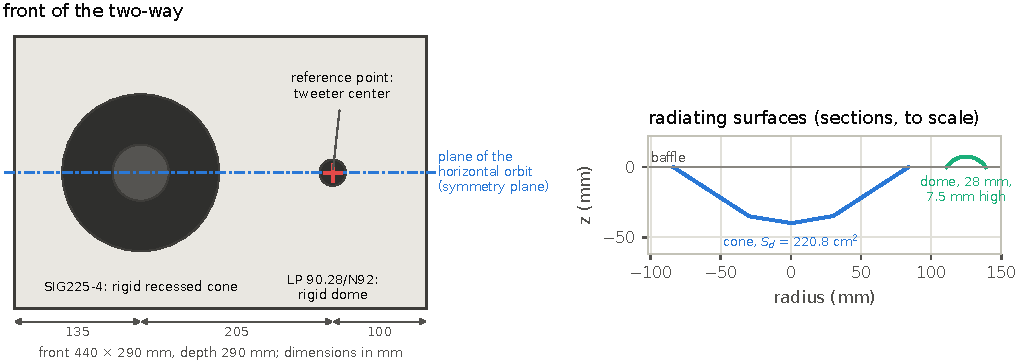
\includegraphics[width=\textwidth]{bem_model.pdf}
  \caption{The two-way variant solved by the BEM: same cabinet, woofer and tweeter on its horizontal
  middle plane, which is the plane of the horizontal orbit and a plane of symmetry.}
  \label{fig:bemmodel}
\end{figure}

\paragraph{Drivers.} For each driver moving with a volume velocity of 1\,m$^3$/s, the BEM gives the
complex pressure $Z_i(\vect M,f)$ at any point $\vect M$ (Pa per m$^3$/s). The volume velocity comes
from the datasheet response of Section~\ref{sec:datasheets} (the woofer in its 24\,L box):
\begin{equation}
  p_i(\vect M,f)=U_i(f)\,Z_i(\vect M,f),\qquad U_i(f)=\frac{H_i(f)}{q_i(f)},\qquad
  q_i(f)=\frac{\jj\omega\rho_0}{2\pi r_\text{ref}}\,A_i(0,k),
\end{equation}
where $q_i$ is the on-axis far-field pressure of the same radiator in an infinite baffle per unit
volume velocity, according to the aperture model of Eq.~\eqref{eq:dome} (with the cone's profile
$z(r)<0$ for the woofer). Were that model exact, $p_i$ would be $H_i\,D_i(\theta,k)\,(r_\text{ref}/r)\,
e^{-\jj kr}$ in an infinite baffle, the direct term of Eq.~\eqref{eq:ded}: the BEM and the DED model of
this two-way share the same drivers and differ only by how they radiate and diffract. The DED model
is evaluated with the cone's profile too.

\paragraph{Crossover.} Fourth-order Linkwitz--Riley at 2\,kHz, the woofer high-passed at 40\,Hz, the
filters designed as in Section~\ref{sec:crossover} from the BEM's on-axis responses at 1\,m: the
target times the minimum-phase inverse of each driver's 1/6-octave smoothed magnitude. The same
filters serve both models.

\subsection{The boundary-element solution}

The BEM data were computed with Huygens, a boundary-element solver under development whose code is not
public; the pressures at every microphone position are in the repository
(\texttt{data/bem/two\_way.npz}), with the scripts that turn them into the results below. The method:
\begin{itemize}
  \item exterior Neumann problem of the Helmholtz equation around the closed cabinet, rigid, each
  driver's surface moving along its axis, the other one at rest (one right-hand side per driver);
  \item Burton--Miller formulation \cite{burtonmiller} (the direct integral equation combined with its
  normal derivative, coupling $\alpha=-\jj/k$ for the time factor $e^{+\jj\omega t}$), so that no
  frequency falls on an interior resonance of the box; Galerkin discretization, pressure piecewise
  linear and normal derivative piecewise constant on flat triangles, hypersingular operator in Maue's
  weak form, singular integrals by the Sauter--Schwab transformations \cite{sauter};
  \item uniform mesh of the whole surface, edges of $\lambda/6$ at the top of each band of frequencies
  (bands of a ratio 1.26 in edge length), 50\,mm at most; the half model and its mirror image;
  \item assembly with the near and singular pairs of triangles in double precision on the processor and
  the distant pairs in single precision on the GPU; dense LU factorization in double precision.
\end{itemize}
The \bemFreqs\ frequencies run from 20\,Hz to 16\,kHz in 1/48-octave steps. At 16\,kHz the surface has
\bemTrianglesMax\ triangles and the half model \bemUnknownsMax\ unknowns (\bemGigabytesMax\,GB,
\bemSecondsTop\,s per frequency). The microphone positions are those of the study: the horizontal
orbits of both setups and the vertical orbit of the rigorous setup, at 1\,m and 2\,m, every $5^\circ$
(432 points). The sweep took \bemHours\,h on a Mac mini (Apple M4~Pro, 64\,GB), 62\,\% of it in the top
band.

Two checks on the data. At 20\,Hz, on the 2\,m circle, each driver radiates the pressure of a monopole
of the same volume velocity, $\omega\rho_0 U/(4\pi r)$, to within $\pm7$\,\%, a variation explained below.
Where the mesh changes (by 1.26 in edge length) the levels at the relevant points of the horizontal
orbits move by 0.1 to 0.5\,dB RMS, about as much as from one frequency to the next within a band: the
mesh is fine enough for the comparisons that follow.

All the results of this section are computed at the BEM frequencies for both models, and the power
spectra are smoothed to 1/24 octave as before (on this grid, the mean of three neighboring
frequencies). The evaluation bands are 50\,Hz--4\,kHz for the woofer, 1--16\,kHz for the tweeter and
50\,Hz--16\,kHz for the sum.

\subsection{What the DED model misses}

\paragraph{The low-frequency acoustic center lies ahead of the baffle.} At 50\,Hz the BEM level at
$0^\circ$ exceeds the level at $180^\circ$ by 2.3\,dB at 1\,m and 1.2\,dB at 2\,m: a monopole about
130\,mm in front of the baffle, at both distances --- the low-frequency acoustic center described by
Vanderkooy \cite{vanderkooy2010}. The DED model puts it about 40 to 60\,mm ahead. It is the variation of
the 20\,Hz check above.

\paragraph{Baffle step.} On the reference axis the BEM woofer rises 4.5\,dB above its half-space level
around 1\,kHz, the DED model 2\,dB (Figure~\ref{fig:bemonaxis}).

\paragraph{The dome radiates wider.} The rigid dome of the BEM is much wider than the aperture model of
Eq.~\eqref{eq:dome}: on the tweeter side of the orbit its response falls by 6\,dB at $95^\circ$ at
6.35\,kHz (DED: $75^\circ$), at $80^\circ$ at 10\,kHz ($55^\circ$) and at $50^\circ$ at 16\,kHz ($35^\circ$),
and its on-axis level is 2 to 3\,dB lower above 6\,kHz for the same volume velocity
(Figures~\ref{fig:bemonaxis} and~\ref{fig:bempolars}). The aperture model lets each ring of the cap
radiate as if it lay in a plane baffle; the protruding cap radiates sideways. With the drivers' volume
velocities taken from that model, the BEM tweeter therefore sits 2 to 3\,dB below its datasheet on axis
above 6\,kHz; the crossover's equalization absorbs it.

\paragraph{Stronger diffraction.} More sound reaches the edges, and the BEM's polar patterns carry
interference ripples that the DED model hardly shows. On the woofer side of the front quadrant
($-70^\circ$ to $-20^\circ$) the ripple has a period of about $25^\circ$ at 3\,kHz and $10^\circ$ at
6.35\,kHz, with $\pm1$ to 3\,dB: a secondary source some 330\,mm from the tweeter, the far edge of the
baffle (Figure~\ref{fig:bempolars}). Behind the cabinet the patterns are finer still. Directivity aside
(levels referred to $0^\circ$, Figure~\ref{fig:bemmaps}, Table~\ref{tab:dedvsbem}), the two models differ by
\dvbTwFrontOne\,dB RMS in front of the tweeter and \dvbTwRearOne\,dB behind it at 1\,m.

\begin{figure}[tbp]
  \centering
  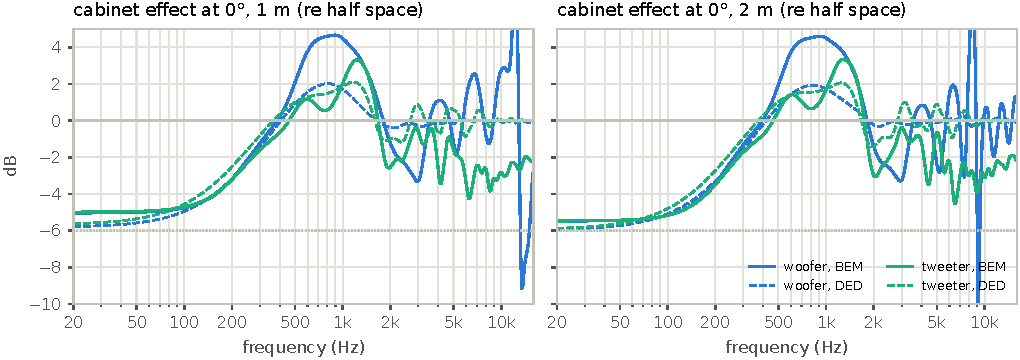
\includegraphics[width=\textwidth]{bem_onaxis.pdf}
  \caption{Each driver at $0^\circ$ (the tweeter's axis), BEM and DED, referred to the same driver in an
  infinite baffle according to the aperture model: the cabinet effect, plus for the BEM the difference
  between the rigid dome and its aperture model above a few kHz. At low frequency the BEM's acoustic center,
  130\,mm ahead of the baffle, raises the level at $0^\circ$.}
  \label{fig:bemonaxis}
\end{figure}

\begin{figure}[tbp]
  \centering
  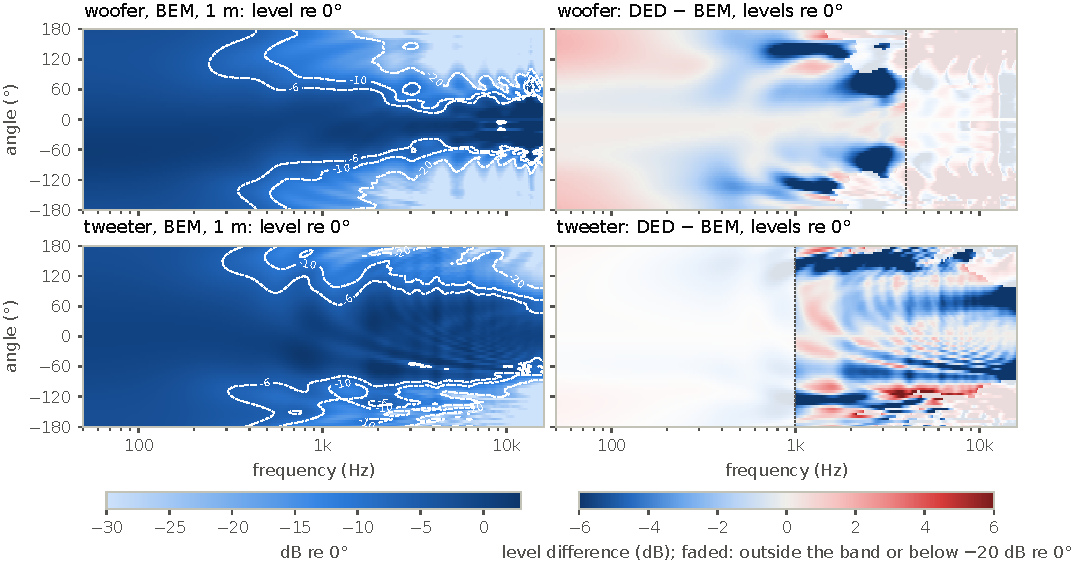
\includegraphics[width=\textwidth]{bem_vs_ded_maps_1m.pdf}
  \caption{Left: BEM polar maps of the two drivers at 1\,m ($5^\circ$ steps), levels re $0^\circ$. Right:
  the DED model's directivity minus the BEM's.}
  \label{fig:bemmaps}
\end{figure}

\begin{figure}[tbp]
  \centering
  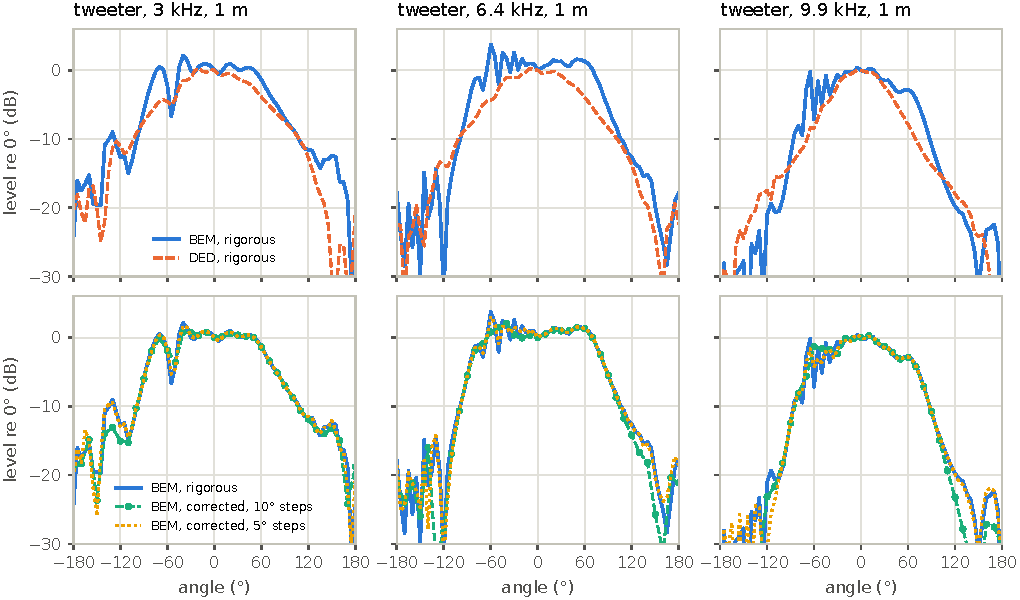
\includegraphics[width=\textwidth]{bem_polars_1m.pdf}
  \caption{Tweeter at 1\,m, level re $0^\circ$ against angle at 3, 6.35 and 10\,kHz. Top: BEM and DED.
  Bottom: what the correction rebuilds from the centered measurements of the BEM, with $10^\circ$ and
  $5^\circ$ steps. Negative angles are on the woofer's side.}
  \label{fig:bempolars}
\end{figure}

\begin{table}[tbp]
  \centering
  \caption{DED against BEM, rigorous setup, levels referred to $0^\circ$: RMS and 95th percentile of the
  difference over the relevant points, in front of the baffle ($|\theta|\le90^\circ$) and behind it (dB).}
  \label{tab:dedvsbem}
  \begin{tabular}{llcccc}
    \toprule
    & & \multicolumn{2}{c}{front} & \multicolumn{2}{c}{behind}\\
    \cmidrule(lr){3-4}\cmidrule(lr){5-6}
    $d$ & & RMS & P95 & RMS & P95\\
    \midrule
    \rows{bem_dedvsbem}
    \bottomrule
  \end{tabular}
\end{table}

\subsection{The correction on the BEM data}

Table~\ref{tab:bemerrors} and Figures~\ref{fig:bemerrmaps} and~\ref{fig:bemresiduals} give the
residuals; Table~\ref{tab:bemcta} the spatial averages.

\paragraph{The woofer} is corrected as well as in the DED model of this two-way: \bemWfCorOne\,dB RMS at
1\,m, \bemWfCorTwo\,dB at 2\,m. The low-frequency acoustic center ahead of the baffle does not get in
the way: the spatial averages of the corrected data stay within 0.03\,dB of the rigorous ones up to
1\,kHz.

\paragraph{The tweeter and the summed loudspeaker} keep more than in the DED model: \bemTwCorOne\ and
\bemSysCorOne\,dB RMS at 1\,m (DED: \dedTwCorOne\ and \dedSysCorOne\,dB), \bemTwCorTwo\ and
\bemSysCorTwo\,dB at 2\,m. The residual sits where the BEM's patterns are finest: on the woofer's side,
in front and behind, and directly behind the cabinet (Figure~\ref{fig:bemresiduals}). Three mechanisms
add up:
\begin{itemize}
  \item \emph{Angular sampling.} $5^\circ$ steps bring the tweeter to \bemTwFiveOne\,dB RMS at 1\,m and
  \bemTwFiveTwo\,dB at 2\,m, the sum to \bemSysFiveOne\ and \bemSysFiveTwo\,dB.
  \item \emph{Interpolating complex responses.} Where the two measurements that bracket a direction are
  no longer coherent --- the rear patterns at $10^\circ$ steps --- their complex mean cancels in part,
  down to $-20$\,dB notches (Figure~\ref{fig:bempolars}, $-130^\circ$ around 6\,kHz). Interpolating the
  re-propagated powers instead, $|\hat H|^2=\sum_k u_k\,|g_k H_k|^2$ with the phase of the complex
  interpolation, avoids it: \bemTwLevOne\,dB RMS for the tweeter at 1\,m with $10^\circ$ steps,
  \bemTwLevFiveOne\,dB with $5^\circ$ (Table~\ref{tab:bemerrors}). In the DED model it makes no
  difference.
  \item \emph{Secondary sources.} The far edge, 330\,mm from the tweeter, re-radiates the sound that
  grazes the baffle; the correction moves that wave as if it came from the tweeter, so the ripple it
  makes in front lands at the wrong angle. This part remains with $5^\circ$ steps: at 6.35\,kHz the
  corrected response at $-30^\circ$ is 2.2\,dB low with $10^\circ$ steps, 1.1\,dB with $5^\circ$
  (Figure~\ref{fig:bempolars}). It shrinks with distance.
\end{itemize}

\paragraph{Spatial averages.} Up to 3\,kHz the corrected CTA-2034-A curves remain within about 0.1\,dB of
the rigorous ones, as in the DED model. Between 4 and 13\,kHz the residual concentrates in narrow bands:
the PIR deviates by up to \bemPirCorOne\,dB at 1\,m and \bemPirCorTwo\,dB at 2\,m, the listening window by
0.84 and 0.46\,dB (Figure~\ref{fig:bempir}, Table~\ref{tab:bemcta}); uncorrected, the PIR is
\bemPirRawOne\ and \bemPirRawTwo\,dB off. With $5^\circ$ steps the PIR comes within \bemPirFiveOne\,dB
(1\,m), with $5^\circ$ steps and interpolated levels within \bemPirLevFiveOne\,dB. With both orbits, as
the standard measures them, the vertical orbit dilutes the horizontal residual: the PIR is within
\bemPirBothCorOne\,dB at 1\,m and \bemPirBothCorTwo\,dB at 2\,m when only the horizontal orbit needs
correcting (Table~\ref{tab:bemcta2}; the BEM was solved on the rigorous vertical orbit only). In the DED
model, the vertical orbit measured with the loudspeaker on its side and corrected (depth 145\,mm, no
lateral offset) gives a PIR within \dedPirBothCorOne\,dB, from \dedPirBothRawOne\,dB uncorrected.

\paragraph{Parameters.} The conclusions of Section~\ref{sec:variants} stand (Table~\ref{tab:bemvariants}):
an error of $\pm10$\,mm on the depth or on the lateral offset, or of 20\,mm on the distance, changes the
PIR by less than 0.1\,dB; omitting the lateral offset, or giving it the wrong sign, puts the PIR
\bemPirLatZeroOne\ or \bemPirLatSignOne\,dB off at 1\,m, worse than no correction (\bemPirRawOne\,dB).
Crossed over at 2\,kHz instead of 450\,Hz, the woofer needs its own offset more than in the three-way:
without it, \bemWfWfZeroOne\,dB RMS instead of \bemWfCorOne.

\begin{table}[tbp]
  \centering
  \caption{Level error of the two-way, BEM and DED, horizontal orbit: uncorrected, corrected
  ($10^\circ$ steps), corrected with interpolated levels ($10^\circ$), corrected with $5^\circ$ steps (dB,
  over the relevant points).}
  \label{tab:bemerrors}
  \small
  \setlength{\tabcolsep}{4pt}
  \begin{tabular}{lllccccccccccc}
    \toprule
    & & & \multicolumn{3}{c}{uncorrected} & \multicolumn{3}{c}{corrected} & \multicolumn{2}{c}{levels}
    & \multicolumn{2}{c}{$5^\circ$ steps}\\
    \cmidrule(lr){4-6}\cmidrule(lr){7-9}\cmidrule(lr){10-11}\cmidrule(lr){12-13}
    $d$ & model & & RMS & P95 & max & RMS & P95 & max & RMS & max & RMS & max\\
    \midrule
    \rows{bem_errors}
    \bottomrule
  \end{tabular}
\end{table}

\begin{figure}[tbp]
  \centering
  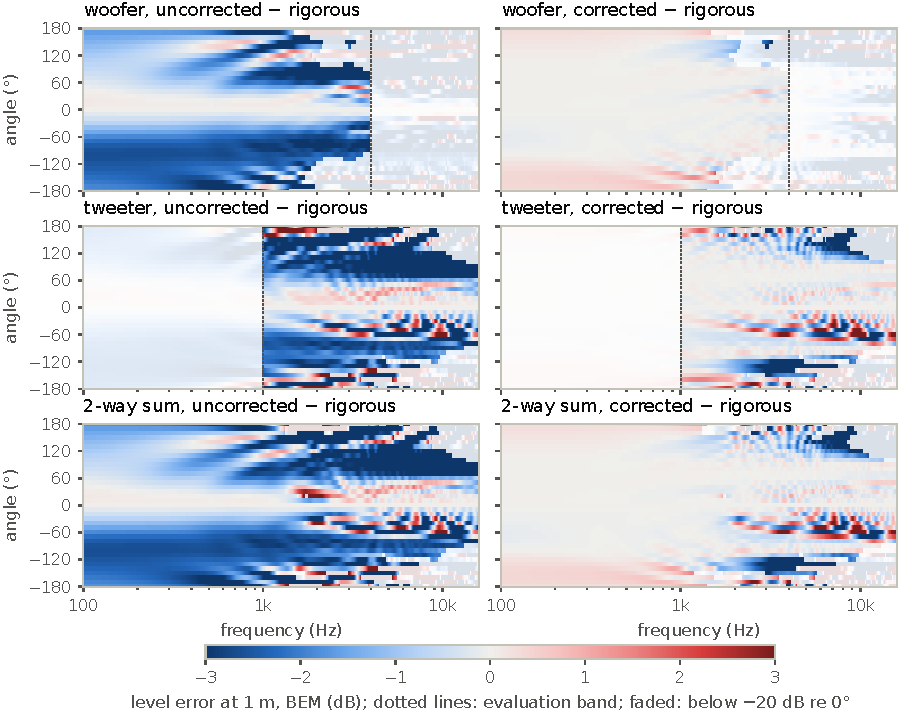
\includegraphics[width=0.92\textwidth]{bem_error_maps_1m.pdf}
  \caption{Level error of the BEM data at 1\,m, uncorrected (left) and corrected (right), $10^\circ$ steps.}
  \label{fig:bemerrmaps}
\end{figure}

\begin{figure}[tbp]
  \centering
  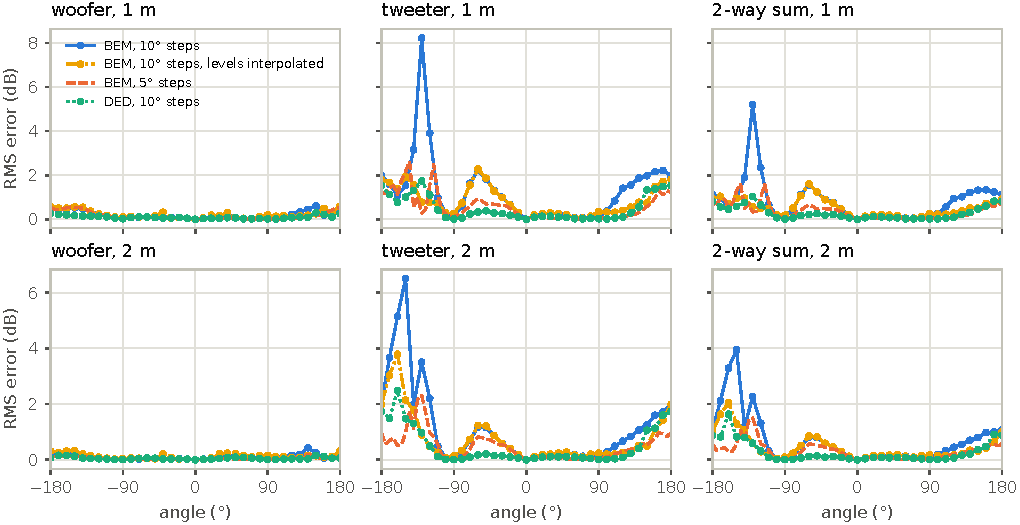
\includegraphics[width=\textwidth]{bem_residuals.pdf}
  \caption{RMS level error of the corrected data at each angle: BEM with $10^\circ$ steps, with interpolated
  levels, with $5^\circ$ steps, and the DED model of the same two-way. Negative angles are on the woofer's
  side.}
  \label{fig:bemresiduals}
\end{figure}

\begin{figure}[tbp]
  \centering
  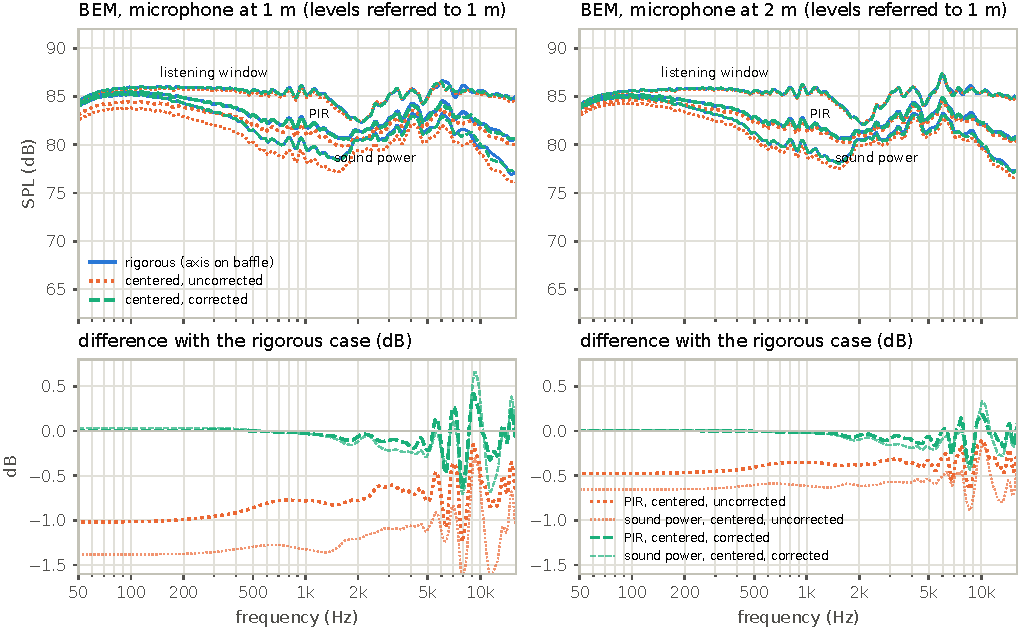
\includegraphics[width=\textwidth]{bem_pir.pdf}
  \caption{Listening window, PIR and sound power of the BEM two-way from the horizontal orbit, and their
  differences with the rigorous case.}
  \label{fig:bempir}
\end{figure}

\begin{table}[tbp]
  \centering
  \caption{Largest deviation from the rigorous case, 100\,Hz--16\,kHz, of the horizontal-orbit
  CTA-2034-A curves of the two-way (dB).}
  \label{tab:bemcta}
  \begin{tabular}{lllccccc}
    \toprule
    $d$ & model & data & LW & ER & SP & PIR & DI\\
    \midrule
    \rows{bem_cta}
    \bottomrule
  \end{tabular}
\end{table}

\begin{table}[tbp]
  \centering
  \caption{The same with both orbits, as CTA-2034-A measures them (dB). BEM: the vertical orbit is the
  rigorous one. DED: the vertical orbit is also measured with the cabinet centered, on its side, and
  corrected.}
  \label{tab:bemcta2}
  \small
  \begin{tabular}{llllcccccc}
    \toprule
    $d$ & model & horizontal & vertical & LW & ER & SP & PIR & SPDI & ERDI\\
    \midrule
    \rows{bem_cta2}
    \bottomrule
  \end{tabular}
\end{table}

\begin{table}[tbp]
  \centering
  \caption{RMS level error and largest PIR deviation of the BEM two-way for the correction variants (dB).}
  \label{tab:bemvariants}
  \small
  \begin{tabular}{lcccc@{\hspace{12pt}}cccc}
    \toprule
    & \multicolumn{4}{c}{1\,m} & \multicolumn{4}{c}{2\,m}\\
    \cmidrule(lr){2-5}\cmidrule(lr){6-9}
    & woofer & tweeter & sum & PIR & woofer & tweeter & sum & PIR\\
    \midrule
    \rows{bem_variants}
    \bottomrule
  \end{tabular}
\end{table}

\paragraph{The two-way's spinorama.} For reference, Figure~\ref{fig:bemspin} shows the CTA-2034-A curves
of the BEM two-way from both orbits at 1\,m.

\begin{figure}[tbp]
  \centering
  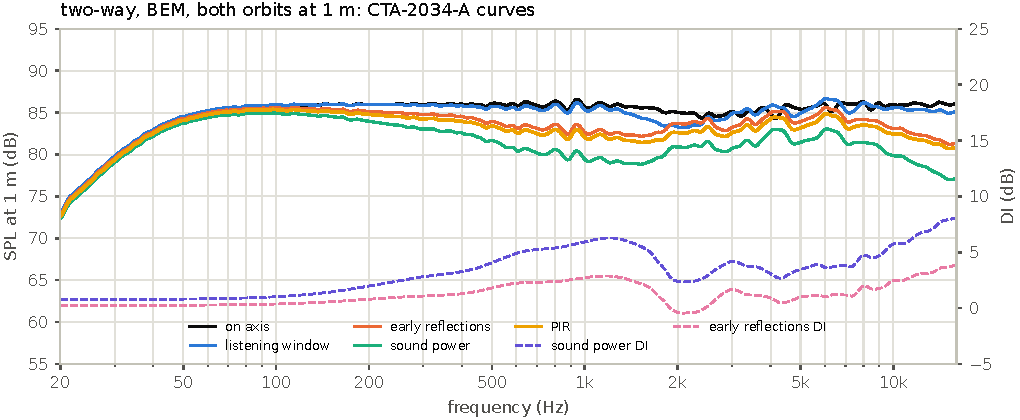
\includegraphics[width=\textwidth]{bem_spinorama.pdf}
  \caption{CTA-2034-A curves of the BEM two-way, rigorous setup, both orbits at 1\,m.}
  \label{fig:bemspin}
\end{figure}

\subsection{What changes}

The BEM confirms what the correction does below about 3\,kHz, where the woofer and the crossover region
are: the spatial averages of the corrected data match the rigorous ones within 0.1\,dB and the lateral
offset is critical. Above, the rigid dome sends more sound to the cabinet's edges than the DED model
assumes, the polar patterns carry finer interference ripples, and the correction leaves more: about
1--2\,dB RMS on the tweeter's individual curves with $10^\circ$ steps, and up to about 0.6\,dB on the PIR
in narrow bands at 1\,m (0.4\,dB at 2\,m). Finer steps and level interpolation recover most of it; the
part due to the far edge remains, smaller at 2\,m.

% =============================================================================================
\section{Discussion}

\paragraph{The geometry is the easy part.} For the direct sound of each driver the correction is
exact up to interpolation, and the angular interpolation of a $10^\circ$ orbit is good enough
(below 0.1\,dB RMS). The out-of-plane offsets between the drivers and the microphone, which the planar
model ignores, do not matter at 1\,m.

\paragraph{Diffraction is the limit, mostly behind the cabinet.} The edge waves come from the baffle
edges, not from the driver; the correction re-times them as if they did. In this simulation the
consequence is small in front of the loudspeaker and grows behind it, at mid and high frequencies,
where the edge waves are the response. Spatial averages are barely affected: the PIR of the corrected
data is within about 0.1\,dB of the rigorous one. Individual rear curves can show local deviations of a
few dB in narrow bands. The boundary-element
check (Section~\ref{sec:bem}) shows that the DED model underestimates that diffraction for a dome
tweeter: the rigid dome radiates wider, more sound reaches the edges, and the residual grows above
3\,kHz, in front on the side of the far edge as well as behind --- up to about 0.6\,dB on the PIR in
narrow bands at 1\,m. Below 3\,kHz the BEM confirms the DED results.

\paragraph{1\,m or 2\,m.} At 2\,m the raw errors are halved and the finite-distance part of the
diffraction error shrinks, but the angular-interpolation part does not; a finer orbit
($5^\circ$) is then the effective remedy. In a real room the choice is also about the reflection-free
time window, which shrinks with distance --- outside the scope of this free-field study.

\paragraph{Interpolate levels.} Where the angular step undersamples the pattern, the two measurements
that bracket a direction are not coherent and the linear interpolation of complex responses cancels in
part, with artificial notches. Interpolating the re-propagated powers, keeping the phase of the complex
interpolation, removes them; on the BEM data it halves the residual of the tweeter with $10^\circ$ steps
and costs nothing where the data are well sampled.

\paragraph{The lateral offset is the trap.} The model handles the laterally shifted microphone,
provided the lateral offset is entered, with the right sign. A wrong or missing lateral offset is
worse than no correction. A quick check: at $+90^\circ$ the microphone must face the side counted as
positive, and the reference axis of a layout like this one lies on that side if the microphone moves
toward the tweeter at positive angles.

\paragraph{Limits of the study.}
\begin{itemize}
  \item Free field. The room, the gating window and its interaction with the correction (the delays
  change by up to 1\,ms behind the cabinet) are not simulated.
  \item The DED model is an approximation: only the edges of the front baffle are modelled, the field
  behind the cabinet is the sum of the edge dipoles, and the edges are sharp. The boundary-element check
  removes the first two approximations for a two-way variant and finds more diffraction above 3\,kHz.
  Real cabinets with rounded edges diffract less, which should help the correction.
  \item Rigid pistons, cones and domes. Real diaphragms break up at high frequency and real tweeters sit
  in faceplates or waveguides, which change their directivity and how much sound reaches the edges.
  The acoustic centers are on the baffle plane: a real acoustic center behind or in front of the baffle
  acts like a depth error for that driver; $\pm10$\,mm of depth error costs little here, and the
  low-frequency acoustic center, 130\,mm ahead of the baffle in the BEM, does not disturb the
  correction.
  \item The vertical orbit, measured with the loudspeaker on its side, was simulated for the two-way with
  the DED model (depth 145\,mm, no lateral offset; Table~\ref{tab:bemcta2}), the BEM on the rigorous
  vertical orbit only. The three-way's CTA-2034-A curves are horizontal-orbit estimates.
\end{itemize}

\begin{tcolorbox}[colback=gray!4,colframe=gray!45,title=Checklist for a small-turntable polar measurement,fonttitle=\bfseries\small,fontupper=\small]
\begin{enumerate}
  \item Center the cabinet on the turntable; put the microphone on the reference axis (in front of the
  reference point) at $0^\circ$, at the reference height.
  \item Measure the depth (rotation axis to baffle) and the lateral offset (rotation axis to reference
  axis) to within about 1\,cm; note on which side the microphone faces at $+90^\circ$ and give the
  lateral offset that sign.
  \item Give every driver its offset from the reference axis in the plane of rotation --- a woofer
  beside the tweeter in a horizontal cabinet is not at 0.
  \item Use $5^\circ$ steps if the responses above a few kHz matter, behind the cabinet and on the side
  of the far edge, and interpolate levels rather than complex responses.
  \item Treat rear responses at mid and high frequencies as approximate (cabinet diffraction). Spatial
  averages (sound power, PIR, DI) are robust: within about 0.1\,dB below 3\,kHz, a few tenths of a dB
  in narrow bands above.
\end{enumerate}
\end{tcolorbox}

% =============================================================================================
\section{Conclusion}

On a small turntable the cabinet is centered and the microphone moved sideways to face the reference
point; uncorrected, the off-axis data are too low (up to 2.5\,dB behind the cabinet at 1\,m), late and
seen from the wrong direction, and the PIR is about 1\,dB low. A geometric correction --- each driver a
point source with directivity, re-propagated and interpolated --- restores them: essentially exactly
for the direct sound, and to within a few tenths of a dB RMS once the cabinet's edge diffraction is
included, the residual being concentrated behind the cabinet at mid and high frequencies. The spatial
averages of CTA-2034-A, PIR included, come within about 0.1\,dB of the rigorous ones. A boundary-element
solution of a two-way in the same cabinet confirms this below about 3\,kHz; above, the dome tweeter
drives the cabinet's edges harder than the edge model assumes, and the corrected PIR deviates by up to
about 0.6\,dB in narrow bands at 1\,m (0.4\,dB at 2\,m), 0.3\,dB with $5^\circ$ steps and interpolated
levels. The method is only as good as its parameters, and one of them is critical: the lateral offset of
the reference axis, with its sign.

\appendix

\section{Additional figures}

\begin{figure}[htbp]
  \centering
  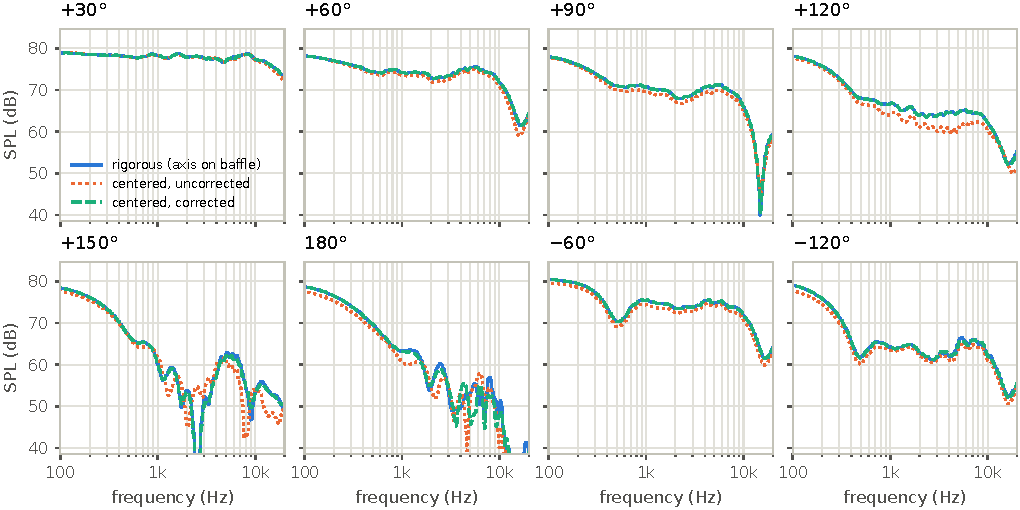
\includegraphics[width=\textwidth]{selected_system_2m.pdf}
  \caption{Summed loudspeaker at selected angles, 2\,m (levels at 2\,m), 1/12-octave smoothing.}
  \label{fig:selected2}
\end{figure}

\begin{figure}[htbp]
  \centering
  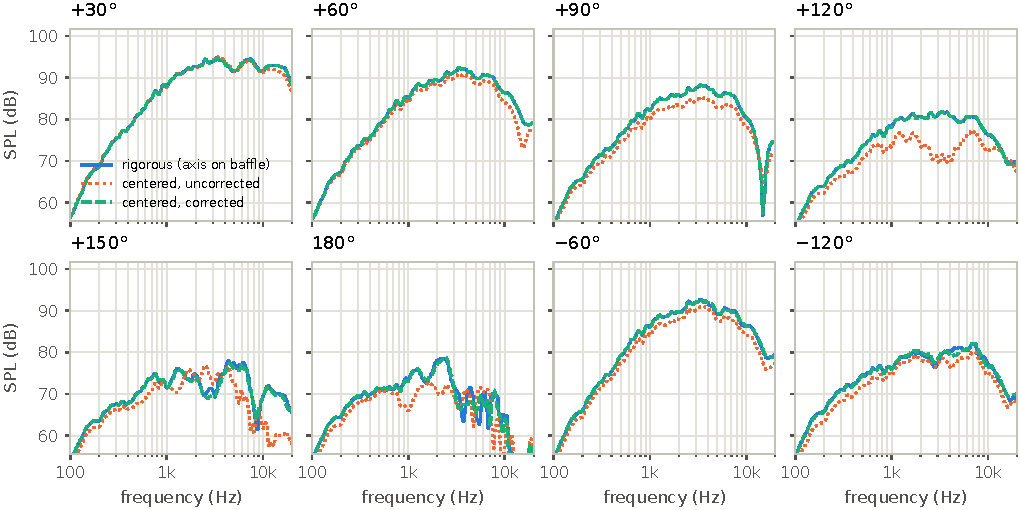
\includegraphics[width=\textwidth]{selected_tweeter_1m.pdf}
  \caption{Tweeter alone at selected angles, 1\,m, 1/12-octave smoothing. Behind the cabinet the
  response is made of edge waves; the corrected curves follow the rigorous ones with local
  deviations in the 4--8\,kHz ripple.}
  \label{fig:selectedtw}
\end{figure}

\FloatBarrier
\section{Reproducibility}

Everything in this report is produced by the Python code of the repository (NumPy, SciPy, Matplotlib),
from the boundary-element pressures for Section~\ref{sec:bem}:
\begin{itemize}
  \item \texttt{rotcenter/}: geometry and kinematics, radiators, driver models, DED diffraction, the
  correction (time and frequency domains), CTA-2034-A averages (one or both orbits), crossovers,
  metrics, the two-way variant;
  \item \texttt{scripts/run\_study.py}: all simulated measurements of the three-way ($\approx$\,5\,min);
  \item \texttt{data/bem/}: the BEM pressures of the two-way (\texttt{two\_way.npz}: each driver,
  per unit volume velocity, at the 432 microphone positions of \texttt{points.json} and the \bemFreqs\
  frequencies, with the mesh size and the time of each solve), and \texttt{scripts/import\_bem.py}, which
  wrote it from the solver's report;
  \item \texttt{scripts/run\_bem.py}: the two-way, BEM and DED, all cases ($\approx$\,30\,s);
  \item \texttt{scripts/make\_figures.py} and \texttt{scripts/make\_bem\_figures.py}: figures and
  tables;
  \item \texttt{scripts/make\_schematics.py}: the schematics;
  \item \texttt{tests/}: unit tests (kinematics, directivities, DED normalization, correction of an
  ideal point source, time and frequency domains, crossovers, CTA-2034-A curves, the two-way's
  microphone positions against the BEM data).
\end{itemize}
The boundary-element solver itself (Huygens) is not public.

The datasheet curves (\texttt{data/datasheets/}) were extracted from the vector graphics of the
manufacturers' PDF datasheets; they belong to their manufacturers and are used here for analysis only.

\begin{thebibliography}{9}
\bibitem{urban2004} M.~Urban, C.~Heil, C.~Pignon, C.~Combet, P.~Bauman, ``The Distributed Edge Dipole
(DED) Model for Cabinet Diffraction Effects,'' \emph{J.\ Audio Eng.\ Soc.}, vol.~52, no.~10,
pp.~1043--1059, 2004.
\bibitem{cta2034} ANSI/CTA-2034-A, \emph{Standard Method of Measurement for In-Home Loudspeakers},
Consumer Technology Association, 2015.
\bibitem{vanderkooy1991} J.~Vanderkooy, ``A Simple Theory of Cabinet Edge Diffraction,''
\emph{J.\ Audio Eng.\ Soc.}, vol.~39, no.~12, pp.~923--933, 1991.
\bibitem{beranek} L.~L.~Beranek, T.~J.~Mellow, \emph{Acoustics: Sound Fields and Transducers},
Academic Press, 2012.
\bibitem{sauter} S.~A.~Sauter, C.~Schwab, \emph{Boundary Element Methods}, Springer, 2011.
\bibitem{vanderkooy2010} J.~Vanderkooy, ``The Low-Frequency Acoustic Center: Measurement, Theory, and
Application,'' 128th Convention of the Audio Engineering Society, London, 2010.
\bibitem{burtonmiller} A.~J.~Burton, G.~F.~Miller, ``The application of integral equation methods to the
numerical solution of some exterior boundary-value problems,'' \emph{Proc.\ R.\ Soc.\ Lond.\ A},
vol.~323, pp.~201--210, 1971.
\end{thebibliography}

\end{document}
